% arara: bibtex
\documentclass[12pt,journal]{IEEEtran}			
\usepackage{array,
			booktabs,
			cite,
			enumitem,
			epstopdf,
			fancyhdr,
			float,
			graphicx,
			lipsum,
			lscape,
			mathtools,
			mcode,
			nomencl,			
			parallel,
			rotating,
			soul,
			wrapfig,
			}
\usepackage[final]{pdfpages}
\graphicspath{ {./images/} } % Graphics Path
\bibliographystyle{plain}
\usepackage{listings}
\usepackage{amsmath}

%-------------------------------------
%              ARDUINO
%-------------------------------------

% Arduino style for highlighting
\newcommand\arduinostyle{\lstset{%
    language=C++,
    %otherkeywords={dac,Serial,},
    basicstyle=\footnotesize,% basic font setting
    frame=tb,                         % Any extra options here
    showstringspaces=false            % 
}}

% Arduino Enviornment
\lstnewenvironment{arduino}[1][]
{
\arduinostyle
\lstset{#1}
}
{}

% Arduino for external files
\newcommand\arduinoexternal[2][]{{
\arduinostyle
\lstinputlisting[#1]{#2}}}

% Arduino for inline
\newcommand\arduinoinline[1]{{\arduinostyle\lstinline!#1!}}

\usepackage[utf8]{inputenc}

% Default fixed font does not support bold face
\DeclareFixedFont{\ttb}{T1}{txtt}{bx}{n}{10} % for bold
\DeclareFixedFont{\ttm}{T1}{txtt}{m}{n}{10}  % for normal

% Custom colors
\usepackage{color}
\definecolor{deepblue}{rgb}{0,0,0.5}
\definecolor{deepred}{rgb}{0.6,0,0}
\definecolor{deepgreen}{rgb}{0,0.5,0}

%-------------------------------------
%             PYTHON
%-------------------------------------

% Python style for highlighting
\newcommand\pythonstyle{\lstset{
language=Python,
basicstyle=\ttm,
otherkeywords={self},             % Add keywords here
keywordstyle=\ttb\color{deepblue},
emph={MyClass,__init__,GUI,SerialPort,Error,DataError,ImageError,},          % Custom highlighting
emphstyle=\ttb\color{deepred},    % Custom highlighting style
stringstyle=\color{deepgreen},
frame=tb,                         % Any extra options here
showstringspaces=false            % 
}}


% Python environment
\lstnewenvironment{python}[1][]
{
\pythonstyle
\lstset{#1}
}
{}

% Python for external files
\newcommand\pythonexternal[2][]{{
\pythonstyle
\lstinputlisting[#1]{#2}}}

% Python for inline
\newcommand\pythoninline[1]{{\pythonstyle\lstinline!#1!}}

\setlength\parindent{0.33in}

%-------------------------------------
%       LTPSICE NETLIST
%-------------------------------------

% LTPSICE NETLIST style for highlighting
\newcommand\ltspicestyle{\lstset{
language=Clean, 
basicstyle=\scriptsize
}}


% LTPSICE NETLIST environment
\lstnewenvironment{ltspice}[1][]
{
\ltspicestyle
\lstset{#1}
}
{}

% LTPSICE NETLIST for external files
\newcommand\ltspiceexternal[2][]{{
\ltspicestyle
\lstinputlisting[#1]{#2}}}


\setlength\parindent{0.33in}


%-----------------
% BEGIN DOCUMENT
%-----------------

\begin{document}

% TITLE
\title{The Design and Implementation of a Scanning Fabry-Perot Interferometer for Use in Measuring Multiple Modes in Lasers}

% AUTHOR
\author{David M Houston}

% MAKE TITLE
\maketitle

% ABSTRACT
%-----------------------------------------------------------------------------------------------------------------------------------
\begin{abstract}

A scanning mirror Fabry-Perot Interferometer (sFPI) was designed, built, and implemented to measure the modes of a laser beam. It has an estimated finesse of 522 and free spectral range of 3.75 GHz with a resolution bandwidth of 24 MHz. A piezoelectric device will change the spacing of the mirrors, allowing scanning across multiple free spectral ranges. A voltage-source driver provides a controllable signal to a piezoelectric device. The spectral frequency content will be captured by a photo-detector and amplified by a trans-impedance amplifier. This can be analyzed one of two ways. Either sent to a micro-controller-computer pair which processes, displays, and stores this data locally on a hard disk, or sampled by an oscilloscope which can take the place of the micro-controller.

\end{abstract}
%-----------------------------------------------------------------------------------------------------------------------------------


% KEY WORDS
%-----------------------------------------------------------------------------------------------------------------------------------
\begin{IEEEkeywords}
FSR, sFPI, Python
\end{IEEEkeywords}
%-----------------------------------------------------------------------------------------------------------------------------------


% Introduction Section
%-----------------------------------------------------------------------------------------------------------------------------------
\section{Introduction} \label{ss:introduction}

The current sFPI (Spectra-Physics SP-470-06) is bulky and requires various appendages in order to operate. It requires a separate photodiode and data collection device (i.e. oscilloscope). This makes it cumbersome to use. The new model has been constructed to reduce the overall real estate and make the operation more user friendly. It has a pre-installed photodiode as well as an integrated application which communicates directly with an on-board micro-controller to process and display the spectral content of the cavity. The computer application increases the functionality of the device by calibrating the incoming signal based on user input of the free spectral range of the cavity which prompts the application to mathematically scale the output for analysis. While the newly development sFPI seems to be superior to the other it has its disadvantages. The frequency of the driver is only 2.35 Hz, making it much slower than real-time analysis. It also requires more than one individual to design and build all of the necessary components to make the design successful. 

%-----------------------------------------------------------------------------------------------------------------------------------


% Background section
%-----------------------------------------------------------------------------------------------------------------------------------
\section{Background} \label{ss:background}

In order to understand how the sFPI works, a fundamental principle must be explained. In its static state, a cavity can hold a specific number longitudinal modes, proportional to the length of the cavity ($L$). Verheyen's book on laser electronics gives an adequate definition for a cavity mode:
\\
\begin{quote}
A cavity mode is a field distribution that reproduces itself in relative shape and in relative phase after a round trip through the system~\cite{verdeyen}
\end{quote}
\leavevmode \\
\indent Each mode has an order of the form \textit{(m,n,q)}, where \textit{m, n,} and \textit{q} are integers. The transverse modes are represented by \textit{m} and \textit{n}, and the longitudinal modes are represented by \textit{q}. Typically only the $TEM_{0,0,q}$ modes are examined because it makes the math easier, however higher order transverse modes are prevalent in the system. For our purposes we will only be examining the longitudinal modes. However, when the length of the cavity changes ($\Delta L$), so does the orders of the modes which can occupy length $L+\Delta L$. In order to achieve a maximum transmission, $\Delta L$ must be on the order of a wavelength, corresponding to a $q+1$ increase in the mode order. Any other change in length ($\Delta L$) not on that order will result in little to no transmission of the cavity beam. The separation of the maximum transmission peaks is defined as the free spectral range (FSR) and can be expressed by $\text{FSR}=c/2L$, where \textit{c} is the speed of light in a vacuum. The FSR is described by a frequency, however it can also be related to spacial frequency as well. Figure~\ref{fig:fsr} graphically describes the free spectral range. 

\begin{figure}
	\centering
	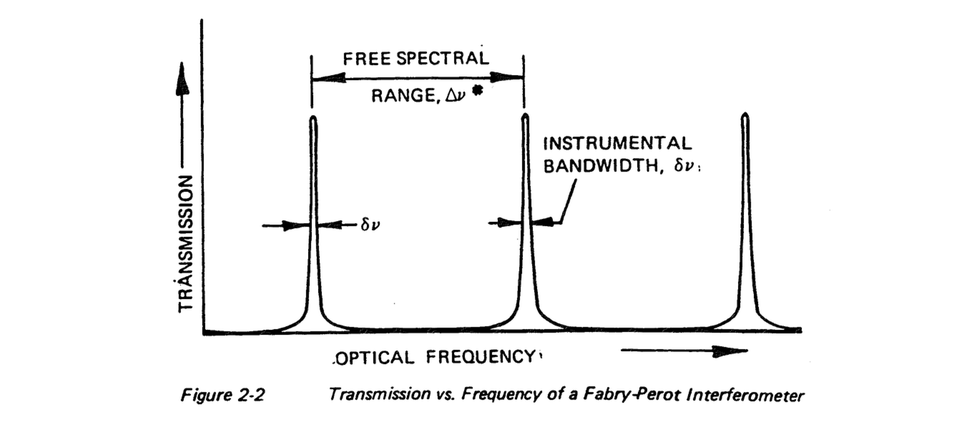
\includegraphics[width=4in]{./FSR_1.png}
	\caption{Spectral Frequency Content of a sFPI~\cite{spectraphysics450}}
	\label{fig:fsr}
\end{figure}

Since this is not a perfect cavity, the photon-lifetime is described by an exponential decay rate, $e^{-t/\tau}$. The line shape of the cavity, which has the shape of a Lorentzian, is the Fourier transform of the photon-lifetime. The line shape is the transmission intensity of the deviations of frequencies from the fundamental. The full-width at half maximum of the line shape is the bandwidth of the cavity. Typically bandwidth is not expressed, but rather the finesse of the cavity. The finesse is defined as the ratio of the free spectral range to the bandwidth of the cavity (Eq.~\ref{eq:finesse}). 

% F = pi / 2asin(1/?F)
\begin{equation}
\mathcal{F} = \frac{\pi}{2sin^{-1}(1/\sqrt{F})}
\label{eq:finesse}
\end{equation}

The finesse is related by a factor defined as the coefficient of finesse ($F$) which is proportional to reflectivity of the mirrors used (Eq.~\ref{eq:cof}).

\begin{equation}
F = \frac{4R}{(1-R)^2}
\label{eq:cof}
\end{equation}  

Dialectically coated mirrors with high reflectivity, at the principle wavelength, are used to increase the finesse and overall performance of the Fabry-Perot cavity. The reflectivity of these mirrors is typically $>90\%$. Since the reflectivity is greater than 50\% the simplified Eq.~\ref{eq:finesse_lth_50} can be used to approximate the finesse. This is because at small values of $x$ for $sin^{-1}(x)$ the relationship is 1 to 1. 

% Equation
\begin{equation}
\mathcal{F} = \frac{\pi R^{1/2}}{1-R}
\label{eq:finesse_lth_50}
\end{equation}   

We have discussed what happens when we change the length of the cavity, but we must further dive into the movement of the cavity. The length of the cavity must be on the order of the principle wavelength to achieve resonance. Thusly, a position change of one wavelength will constitute resonance in the cavity. This insinuates that $\Delta L = n\lambda$, where $\lambda = 632.8 nm$. A piezoelectric device (PED) can generate a $\Delta L$ of that magnitude. While other forms of precision motion control can be used (i.e. pressurized air), a PED's real estate is ideal for the application. A PED's deformation is directly proportional to the electric field applied across it and is related by the following equation, where $x$ is the strain of the PED, $d_{33}$ is the piezoelectric strain constant, and $E$ is the applied electric field~\cite{piezo}. 

% Equation
\begin{equation}
x = d_{33}E
\label{eq:strain}
\end{equation}   

Since strain ($x$) is the ratio of the change in length by the length ($\Delta L/L$) of the material and the applied electric ($E$) is the ratio of the applied voltage ($V$) to the length ($L$) over which it is applied ($V/L$), Equation~\ref{eq:strain} can be expressed as $\Delta L = d_{33}V$, directly relating the change in length to the change in applied voltage~\cite{piezo}. For our applications a sawtooth voltage signal will be applied across the PZT. This will allow for scanning of the mirrors through the modes of the resonant cavity by systematically controlling $\Delta L$ for reproducible output. 

The transmission intensity resulting from the scanning of the cavity by means of the PZT is incident on a photodiode. Photodiodes have a unique characteristic where light incident upon the semiconductor ($h\nu$) produces a current. This can be done in the photo-voltaic or photo-conductive regions of operation; however, the photo-conductive region, which operates in reverse bias, has a much higher responsivity. The responsivity of a photodiode ($R_{\lambda}$) is the ratio of current ($I_{P_n}$) in amperes to the incident power ($P_n$) in watts, where \textit{n} is an integer describing the different levels of incident power (Fig~\ref{fig:diode-curve}). The responsivity can be calculated by Equation~\ref{eq:responsivity}, where $\eta$ is the quantum efficiency, $h$ is Plank's constant, $\nu$ is the frequency of the light, and $e$ is the elementary charge (Eq. ~\ref{eq:responsivity}).    

% Equation
\begin{equation}
R = \eta \frac{e}{h\nu}
\label{eq:responsivity}
\end{equation} 

% IV Diode Curve Figure
\begin{figure}[h!]
	\centering
	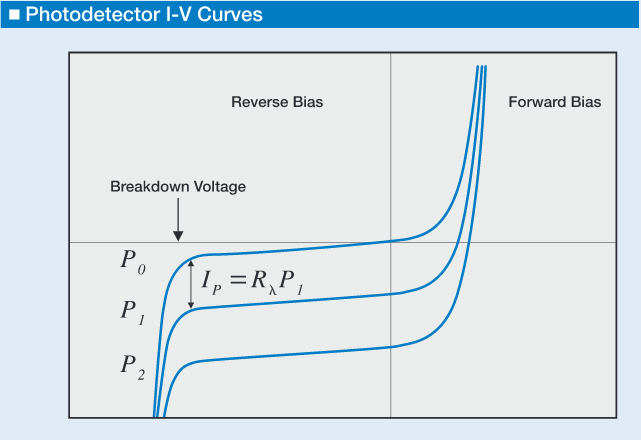
\includegraphics[width=3in]{diode-curve.png}
	\caption{Photo-conductive Diode Curve~\cite{diode-curve}}
	\label{fig:diode-curve}
\end{figure}  

A trans-impedance amplifier can be implemented to convert the current signal into a voltage signal making it quite easy to collect the resulting data using an analog-to-digital converter. However, since the analog-to-digital converter has a limit on the conversion rate, the frequency of the PZT must match this rate to achieve maximum resolution.
%-----------------------------------------------------------------------------------------------------------------------------------


%   sFPI DESCRIPTION
%-----------------------------------------------------------------------------------------------------------------------------------

\section{sFPI Description}

The scanning Fabry-Perot interferometer as discussed in Section~\ref{ss:background} has three main design components: the optical design, the mechanical design, and the electrical design. The cavity design was chosen based on the typical construction for a Fabry-Perot interferometer. The mechanical design was designed for simplicity, with the majority of construction done by a 3D printer. The electrical design was based on the operation of the Spectra Physics Scanning Interferometer Driver which consisted of a signal generator with the ability to tune the amplitude of the signal. This was coupled with a analog-to-computer interface to sample the output of the cavity through a photodiode.  

%-----------------------------------------------------------------------------------------------------------------------------------

% Optical Setup section
%-----------------------------------------------------------------------------------------------------------------------------------

\section{Optical Design} \label{ss:optical_design}

The optical design component, as illustrated in the block diagram, is a Fabry-Perot interferometer. This resonant cavity consists of two spherical mirrors with a radius of curvature equal to 40 mm $\pm\;2$ mm. In order to have a stable cavity the following equation applies.

% 0 ? (1 - L/R1)(1 - L/R2) ? 1
\begin{equation}
0 \leq \Big(1-\frac{L}{R_1}\Big)\Big(1-\frac{L}{R_2}\Big) \leq 1
\label{eq:unsolved_stability}
\end{equation}

Given that $R_1 = R_2 = 40\;\text{mm} \pm2\;\text{mm}$, the range of the length of the cavity ($L$), for a stable resonator, is:

\begin{equation}
0 \leq L \leq 40\;\text{mm} \pm 2\;\text{mm}
\label{eq:cavity_stability}
\end{equation}

The surface of the mirrors are coated with a dielectric material, which has a reflectivity ranging from $99.4-99.8\%$ for 632.8 nm light. The finesse of this cavity, as explained in Section~\ref{ss:background}, is expected to be within the range of $522 - 1569$ for the respective reflectivity.  The resonant cavity for the device is represented in Figure~\ref{fig:resonant-cavity}. 

% Mirror Setup
\begin{figure}[h!]
  \centering
	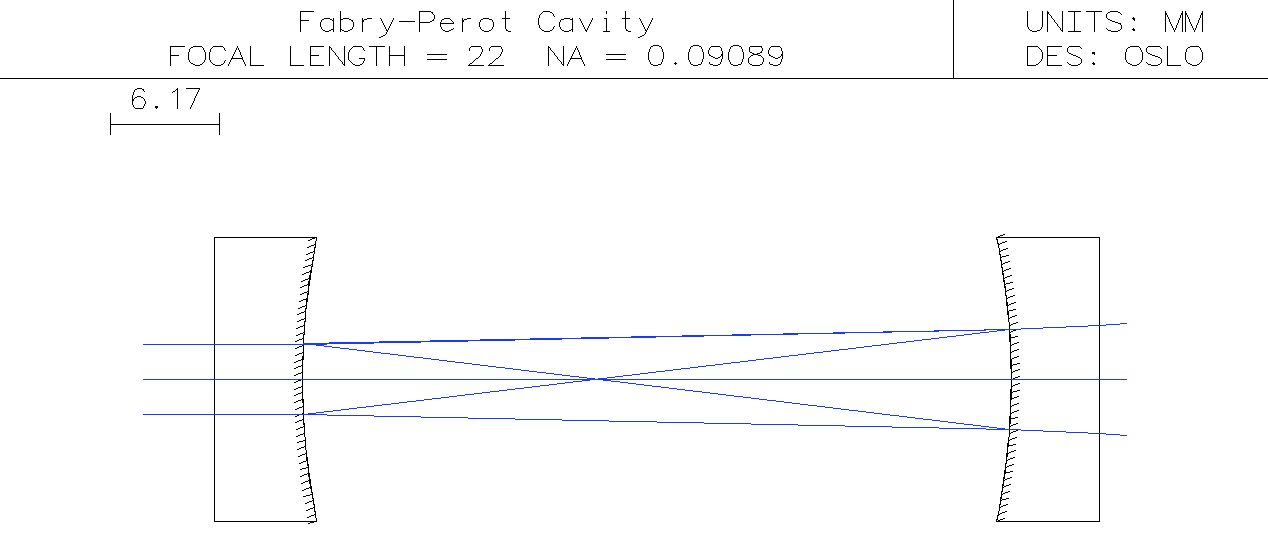
\includegraphics[width=3in]{./cavity/resonant_cavity.png}\\
	\caption[Resonant Cavity Setup]{The resonant cavity is comprised of two dialectically coated spherical mirrors, which reflect 632.8 nm light with ~98\% reflectivity}
	\label{fig:resonant-cavity}
\end{figure}

A 75 mm DCX lens, minimizing spherical aberrations, is used to couple the system and account for any misalignment (Figure~\ref{fig:aux-lens}). By adding in the auxiliary lens the spot size of the output is decreased as well as the divergence angle of the Gaussian beam leaving the cavity. This allows more of the cavity to be used, increasing the photon-lifetime of the cavity. Figures~\ref{fig:mirror-setup} and~\ref{fig:aux-mirror-setup} show the direct improvement of adding in an auxiliary lens to the system. This is done assuming a confocal resonant cavity with the focal point of the auxiliary lens matching the center of the resonant cavity.

% Auxiliary and Resonant Cavity combination
\begin{figure}[h!]
  \centering
	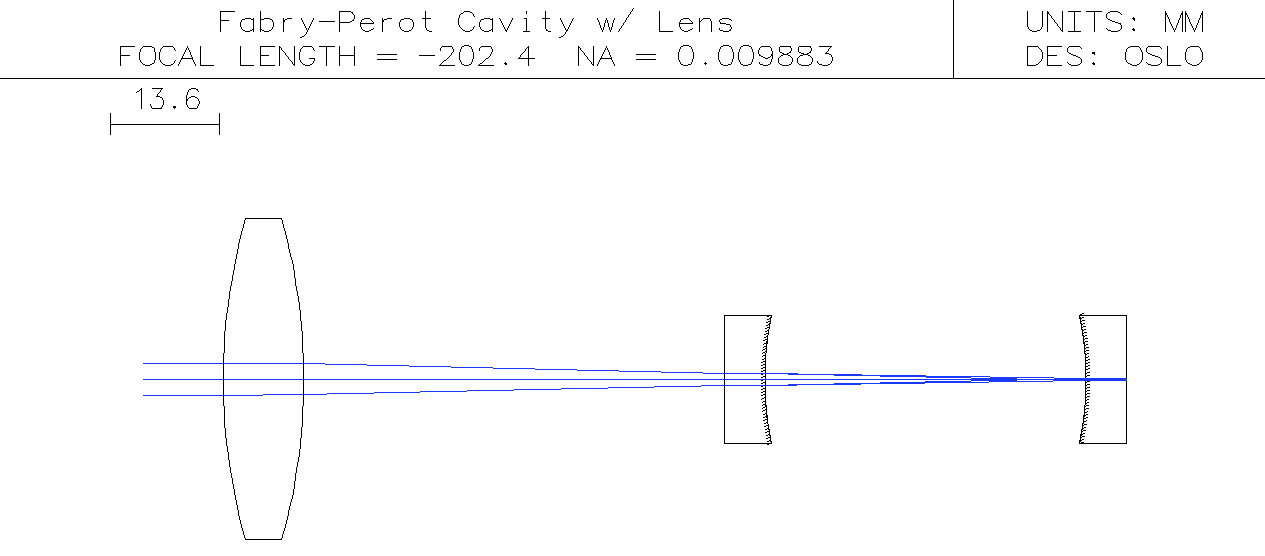
\includegraphics[width=3in]{./cavity/auxiliary_lens_resonant.png}\\
	\caption[Auxiliary Lens Setup]{The auxiliary lens couples the incoming beam to the resonant cavity by increasing the photon-lifetime of the cavity}
	\label{fig:aux-lens}
\end{figure}

% Spot size charts for the cavity with and without the auxiliary lens.
\begin{figure*}[tb]
  \centering
	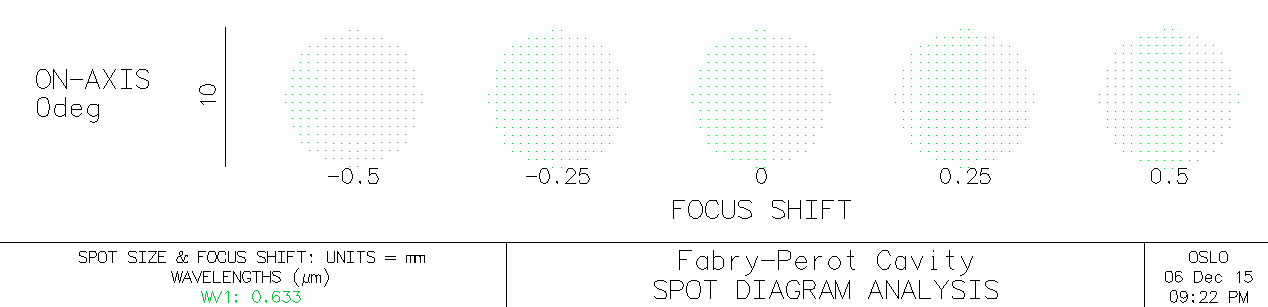
\includegraphics[width=6.5in]{./cavity/spot_size.png}\\
	\caption[Resonant Cavity Setup]{The spot size of the light exiting the resonant cavity after 1 pass}
	\label{fig:mirror-setup}
\end{figure*}

\begin{figure*}[tb]
  \centering
	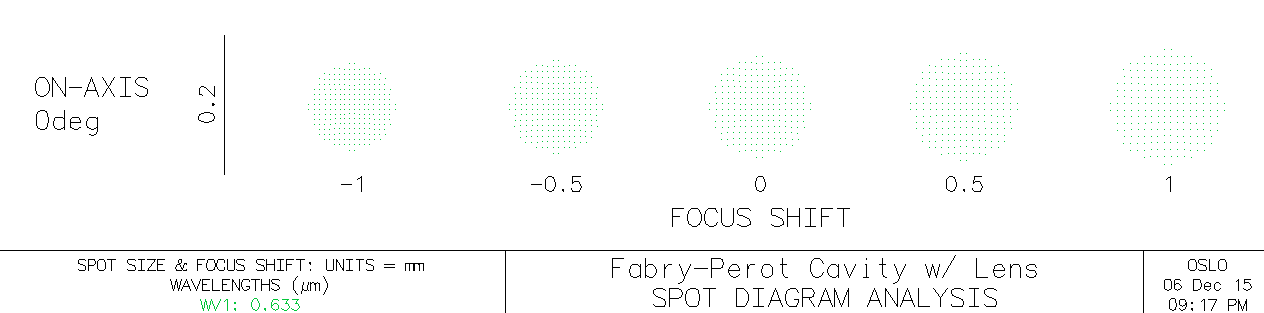
\includegraphics[width=6.5in]{./cavity/auxiliary_lens_spot_size.png}\\
	\caption[Resonant Cavity Setup]{The spot size of the light exiting the resonant cavity after 1 pass with an auxiliary lens of 75 mm focal length}
	\label{fig:aux-mirror-setup}
\end{figure*}


% Mechanical Design
%-----------------------------------------------------------------------------------------------------------------------------------

\section{Mechanical Design} \label{ss:mechanical_design}

The first surface mirror is mounted in a milled disk which is counter sunk, to keep the mirror from falling out (see Figure~\ref{fig:fsm}). This is held in place by a set screw. 

\begin{figure}[h!]
  \centering
	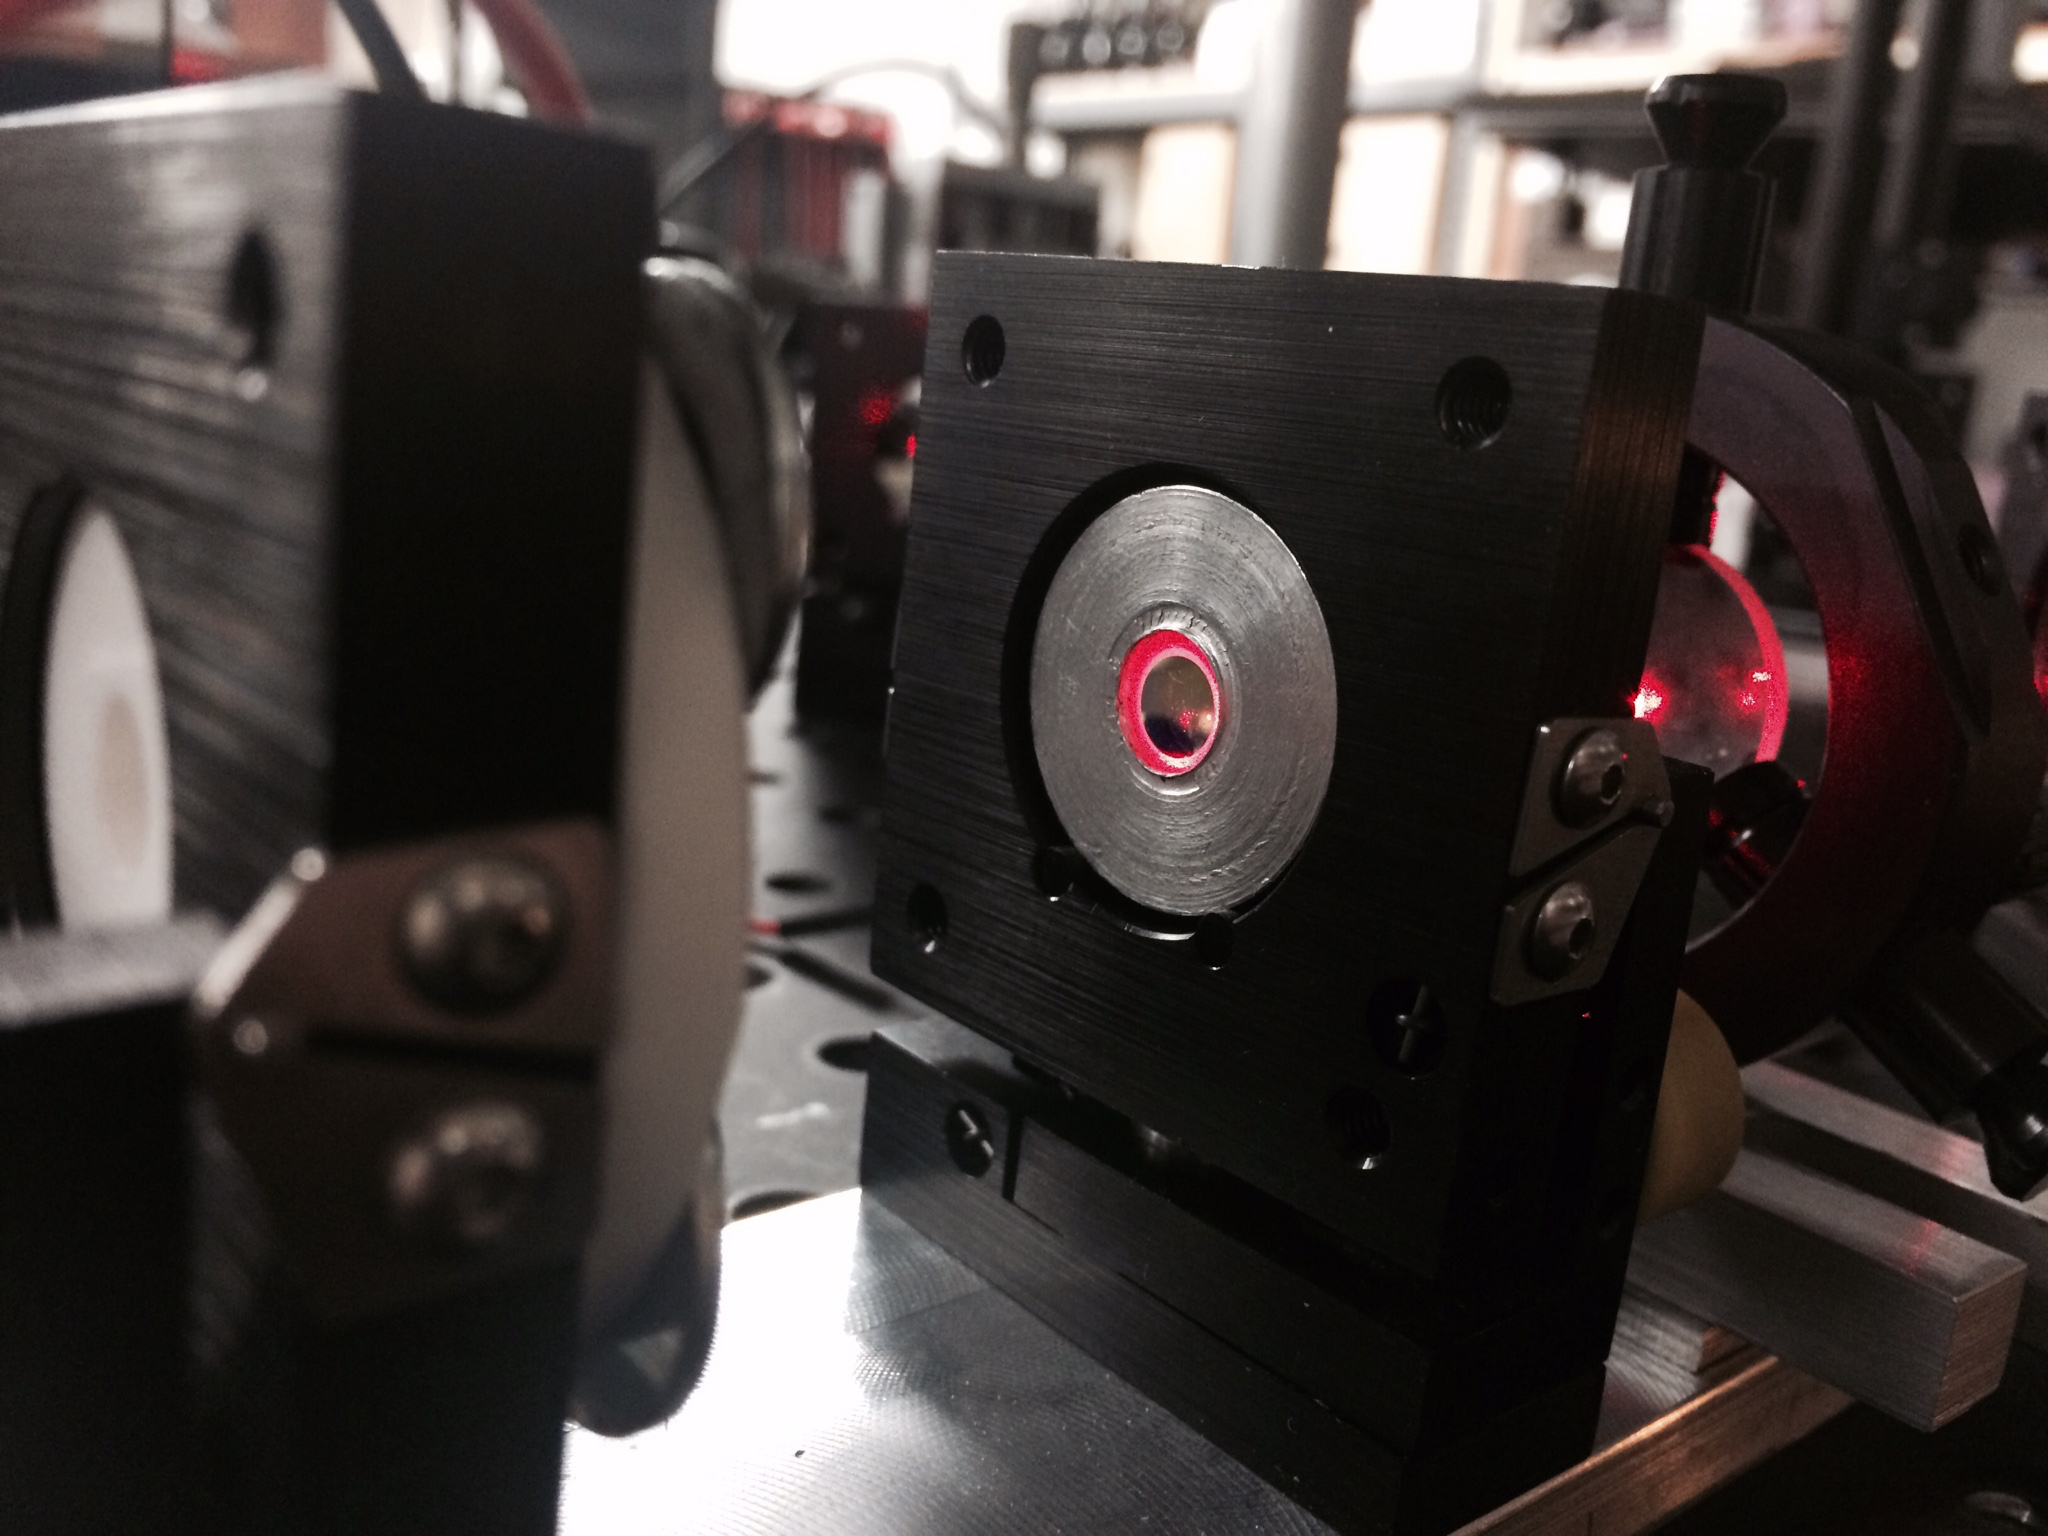
\includegraphics[width=3in]{first-lens-holder.png}
	\caption{Milled Disk for first surface mirror}
	\label{fig:fsm}
\end{figure}

The second surface mirror is attached to the piezoelectric device, which is described in more detail in the next subsection. This is done by the clear adhesive Gorilla Glue. The piezo-mirror combination is mounted to a plastic appendage (Figure~\ref{fig:holder}). When properly aligned, this plastic appendage is designed to keep the limiting aperture within the cavity. It is designed such that 4 washers hold the Piezo-Mirror combination in place, without grounding the plates, and so that it fits inside the adjustable mounts (see Figure~\ref{fig:plastic-mount-piezo-mirror}).  

\begin{figure}[h!]
   \centering
   	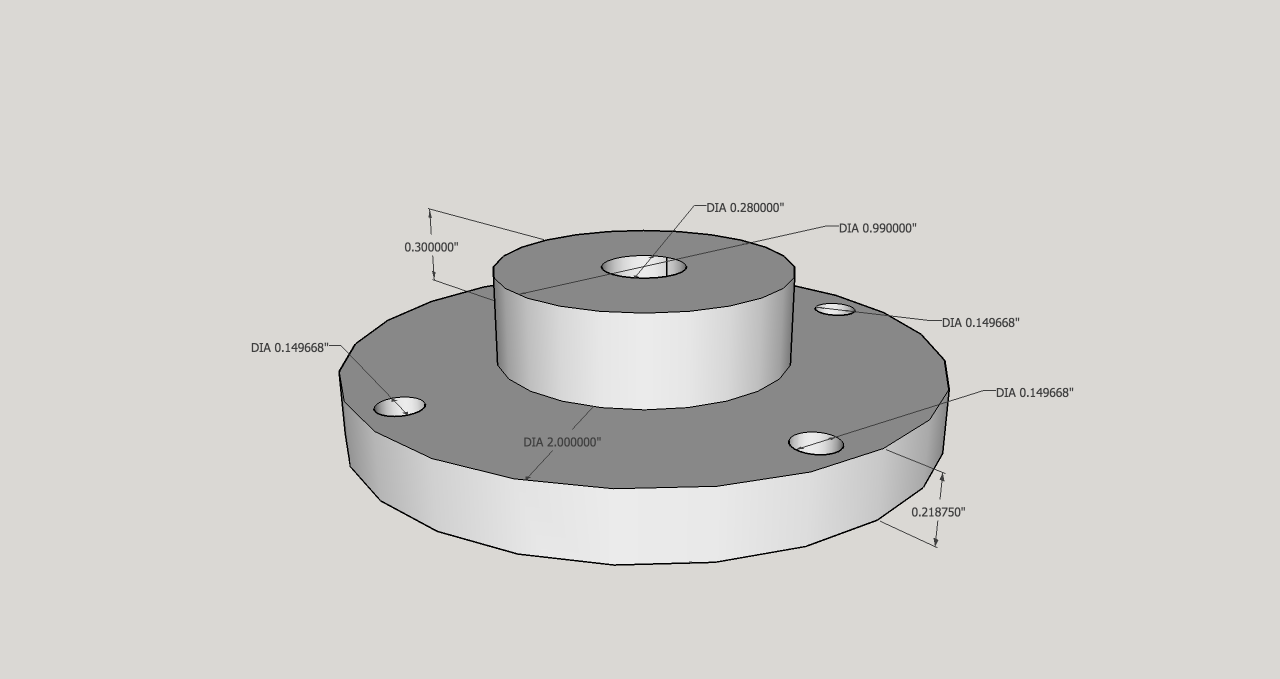
\includegraphics[width=3in]{./mechanical/PZT_holder_3d_rep.png}
	\caption{Piezo-Mirror Holder}
	\label{fig:plastic-mount-piezo-mirror}
\end{figure}

\begin{figure}[h!]
  \centering
	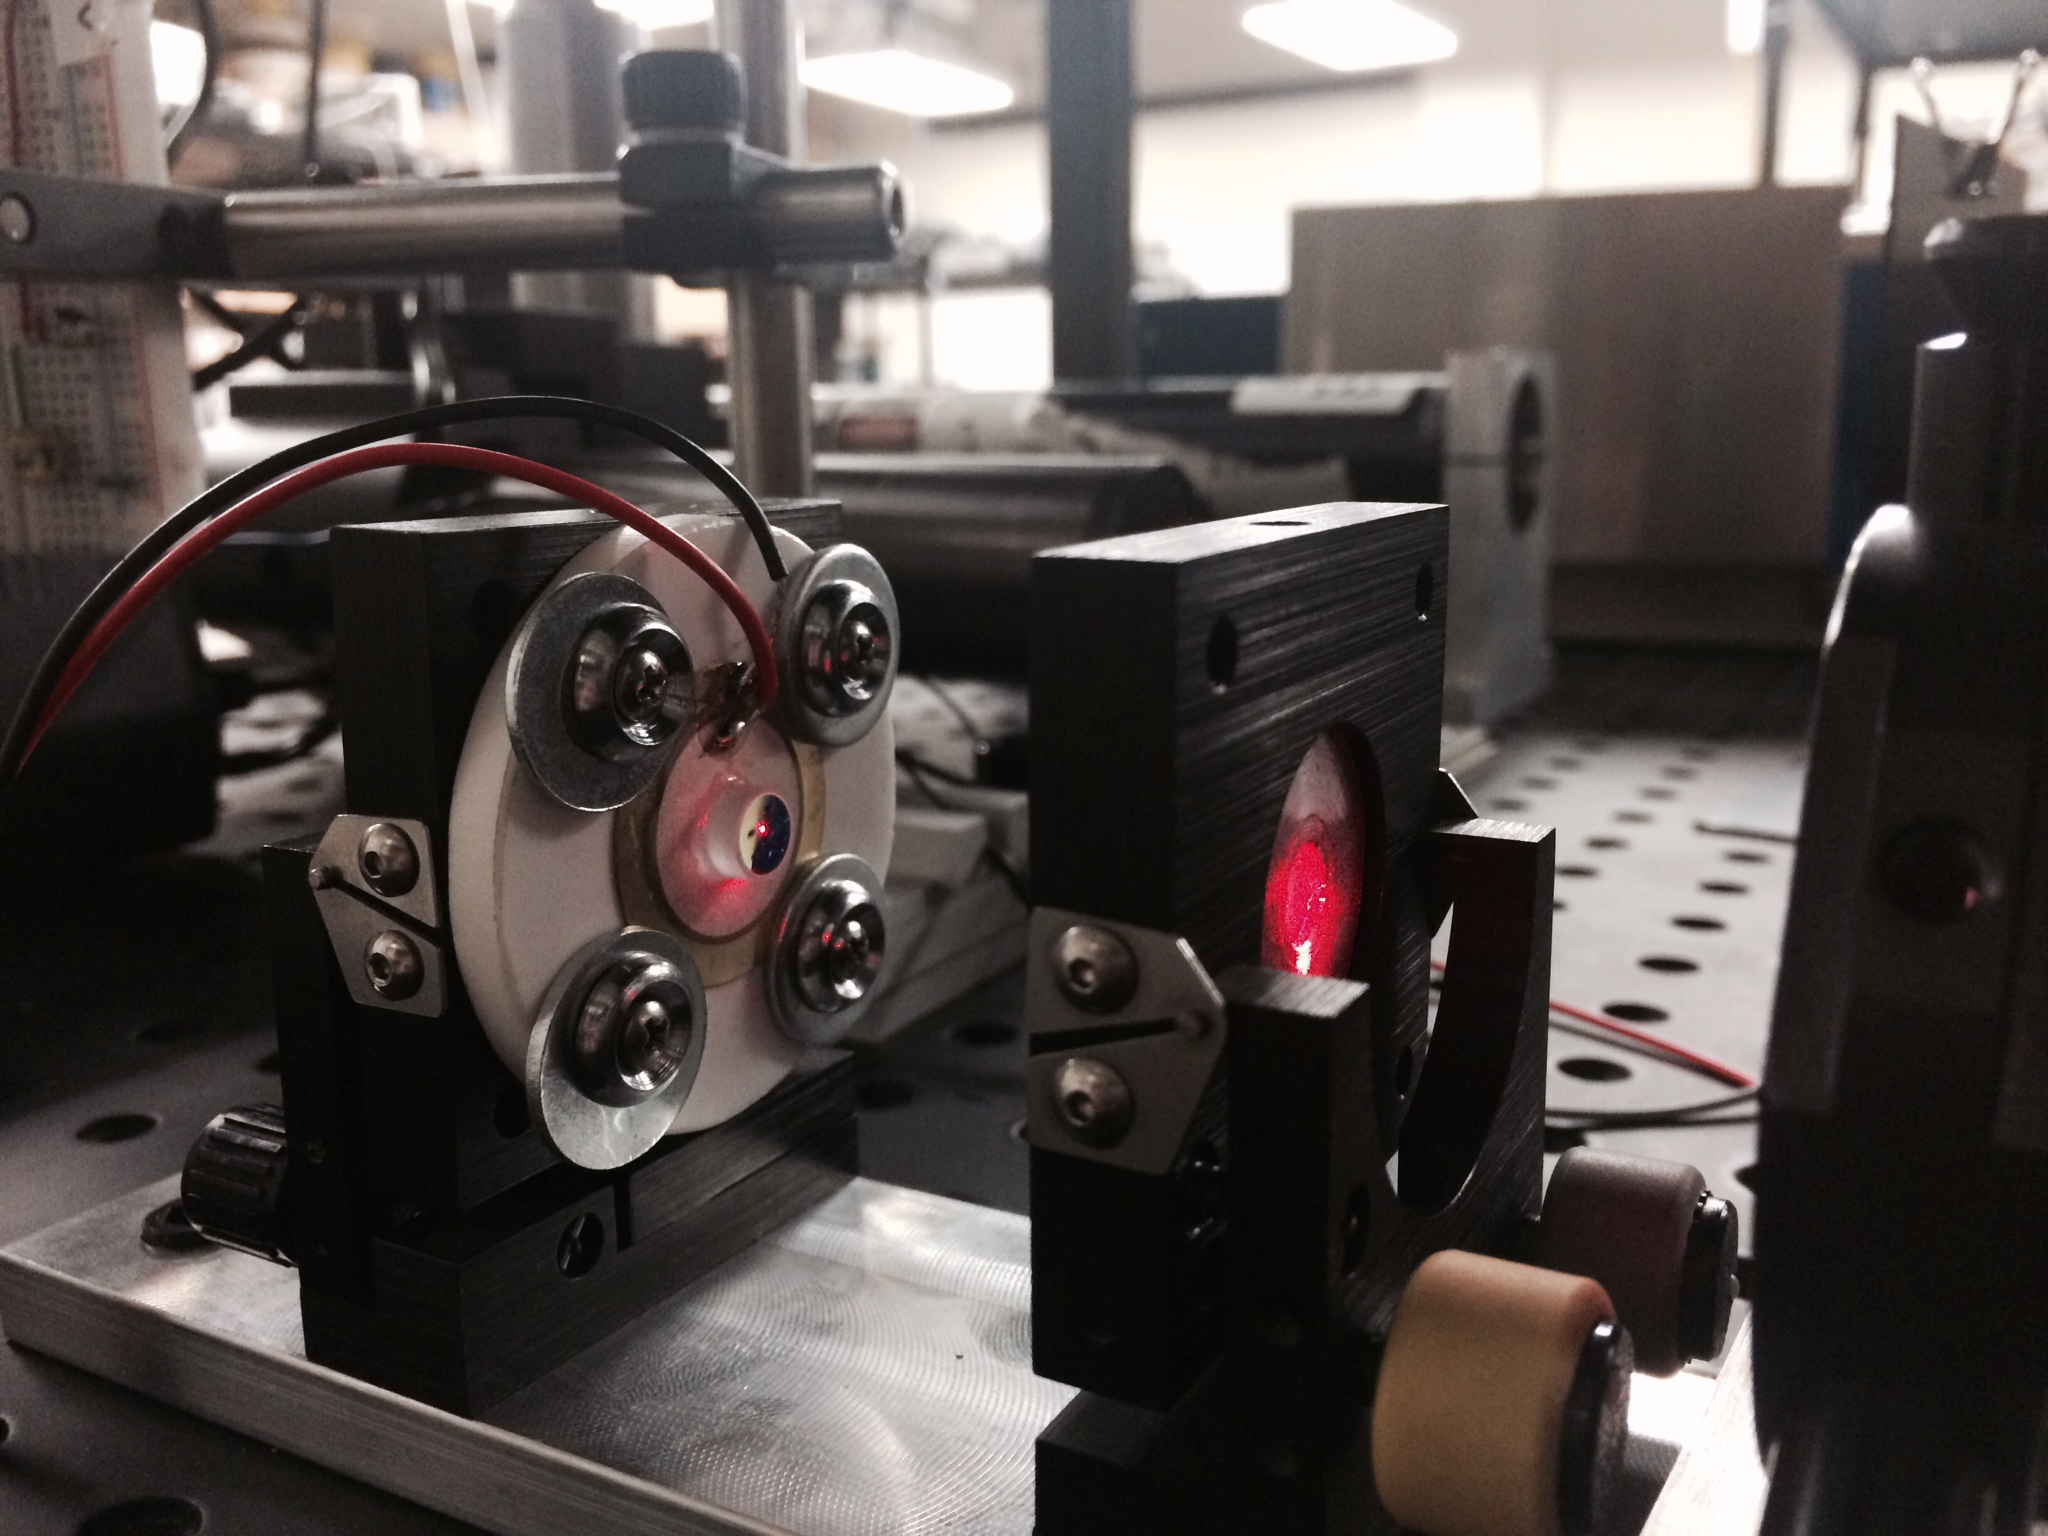
\includegraphics[width=3in]{second-surface-holder.png}
	\caption[Second-Surface Piezo-Mirror Holder]{Piezo-Mirror Holder Dimensions}
	\label{fig:holder}
\end{figure}

The entire cavity is held in place by dual-axis adjustable mounts for aligning purposes (See Figure~\ref{fig:full-cavity}). These are attached to an aluminum base with adjustable distances between the mirrors (Figure~\ref{fig:base}).

\begin{figure}[h!]
  \centering
	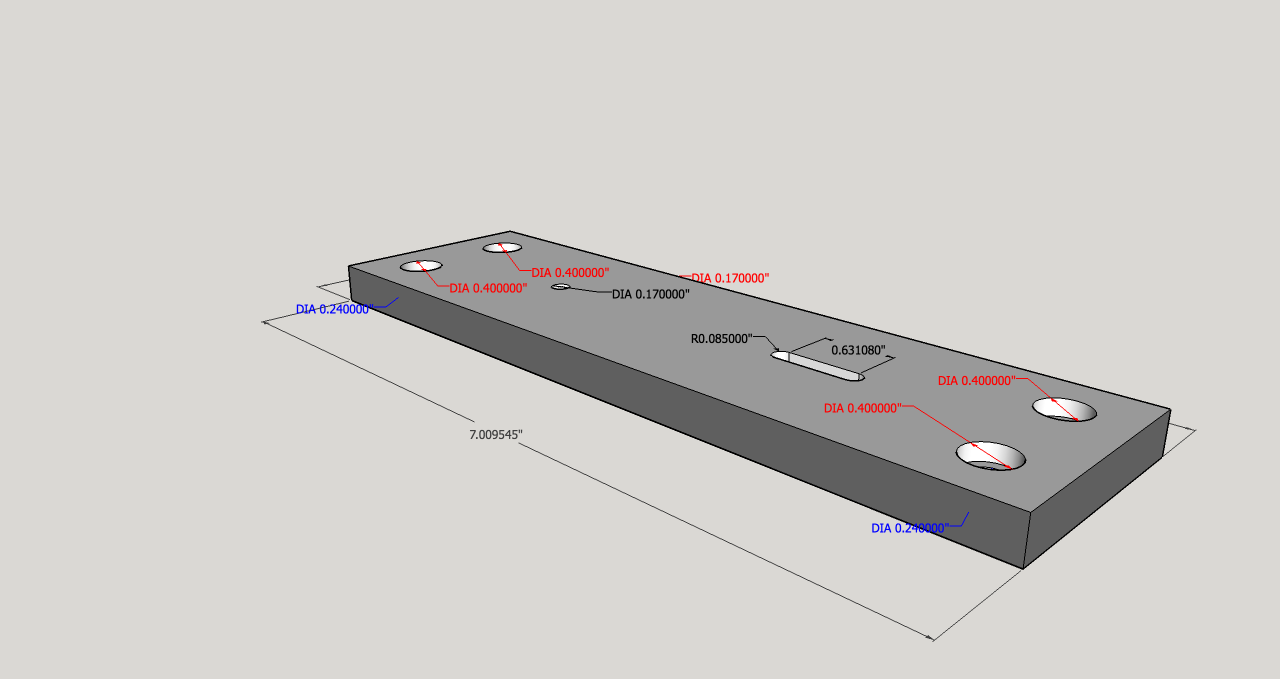
\includegraphics[width=3in]{./mechanical/sfpilensholder_3d_rep.png}
	\caption[Cavity Mounts]{Aluminum base for the sFPI cavity system. Full layout drawings with measurements can be found in on page~\pageref{ss:sfpilensholder}}
	\label{fig:base}
\end{figure}

\begin{figure}[h!]
  \centering
	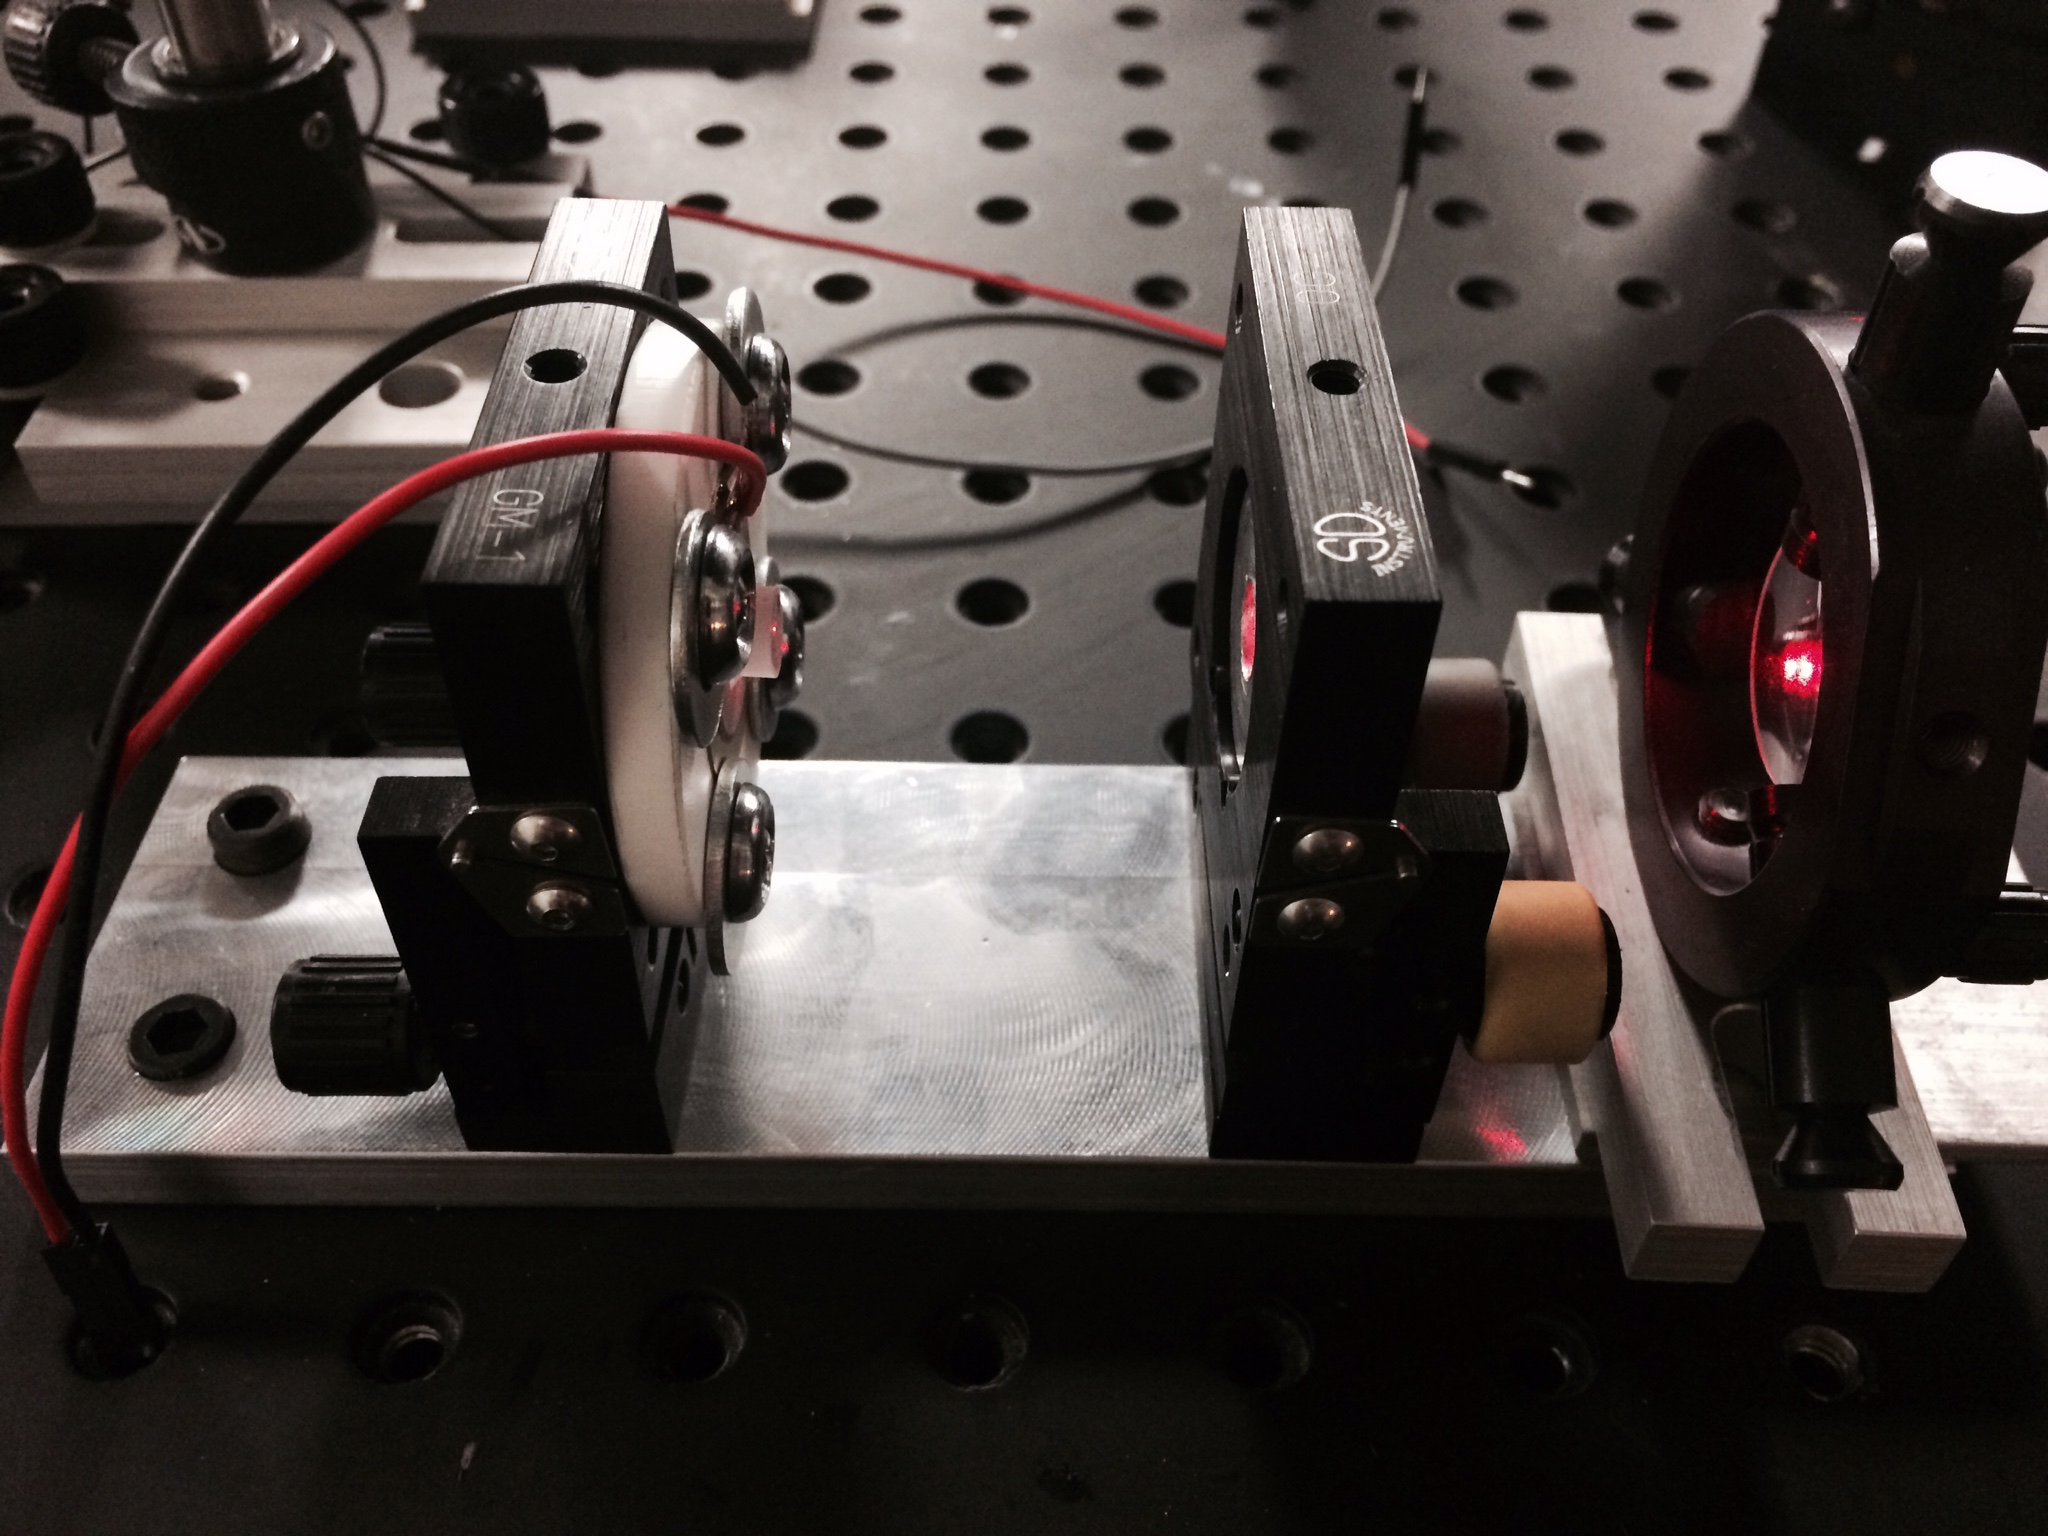
\includegraphics[width=3in]{full-cavity.png}
	\caption[Cavity Mounts]{Adjustable mounts for entire cavity setup}
	\label{fig:full-cavity}
\end{figure}

The photodiode is mounted on the back of the adjustable mounts by the specially made holder (Figure~\ref{fig:diode_holder}). A set screw is taped post-3D-print in order to secure the photodiode. This is done with a 4-40 drill and tap for a 4-40 set screw. 

\begin{figure}[h!]
  \centering
	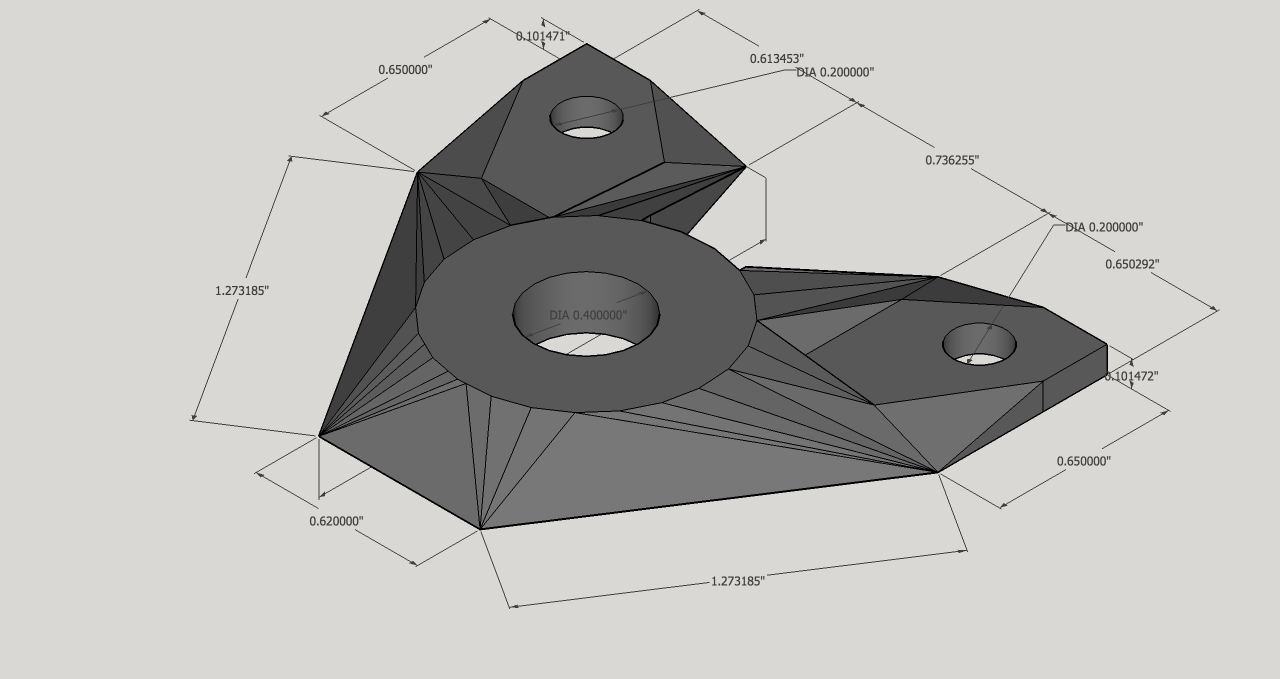
\includegraphics[width=3in]{./mechanical/diode_holder_3d_rep.png}
	\caption[Cavity Mounts]{The mounting device for the photodiode with all measurements and outlays specified on page~\pageref{ss:diode_holder}}
	\label{fig:diode_holder}
\end{figure}

\begin{figure*}[tb]
  \centering
	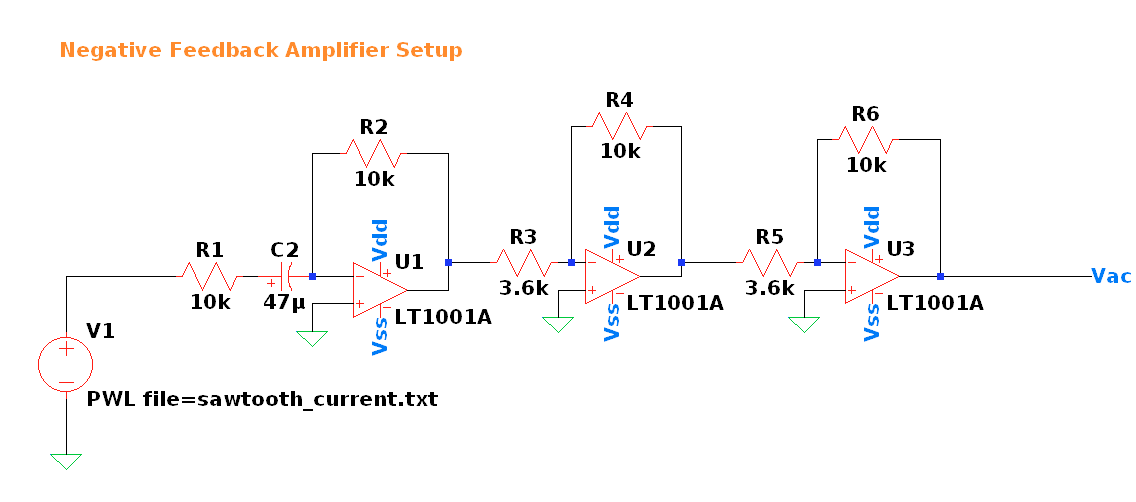
\includegraphics[width=6in]{/ltspice/amplifier-circuit-design-ltspice.png}
	\caption{The three-stage negative feedback amplifier configuration provides a range of 0.5 V/V up to 9 V/V of amplification to the input signal by changing resistors R3 and R5 from $3.3\;k\Omega$ to $10\;k\Omega$ and R1 from $10\;k\Omega$ to $100\;k\Omega$. $V_{DD}$ and $V_{SS}$ are the respective positive and negative voltage rails +17V and -17V.}
	\label{fig:amplifier-configuration}
\end{figure*}
%-----------------------------------------------------------------------------------------------------------------------------------


% Driver Design
%-----------------------------------------------------------------------------------------------------------------------------------

\section{Interferometer Driver Design}

%---------------------
% Piezo Electric Device
%---------------------

\subsection{Piezo-Electric Device}

As stated in the previous sections, when a voltage difference is applied across a piezoelectric device a deformation occurs. This results in an overall change in length ($\Delta L$) of the piezo. In order to properly design the function generator, which will be driving the PZT, a Michelson Interferometer was constructed (see Figure~\ref{fig:michelson-interferometer}) to determine the strain coefficient of the material. 

\begin{figure}
\centering
	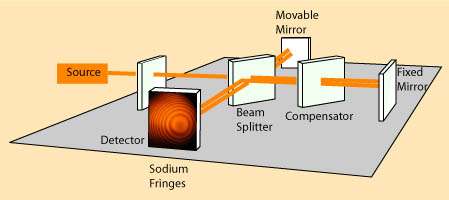
\includegraphics[width=3in]{./michelson.png}
	\caption[Michelson Interferometer]{Michelson Interferometer used for precisely measuring the change in distance of the piezoelectric device per voltage differential placed across it~\cite{michelson}}
	\label{fig:michelson-interferometer}
\end{figure}

The PZT was supplied with an adjustable voltage supply ranging from 0-30V. When cycling from 0 to 30 V, seven individual fringe movements occurred. The distance moved was calculated to be:

\begin{equation}
d = \frac{m\lambda}{2} = 2.2 \;\mu \text{m}
\end{equation}

Where $\lambda$ is the wavelength of the light (632.8 nm) and $m$ is the number of fringe changes observed. This resulted in the piezoelectric strain constant ($d_{33}$) equivalent to $73 \;\text{nm/V}$. With a voltage scan from 0-30V will produce roughly 3.5 free spectral ranges when used in the sFPI. Based on this data, the PZT is adequate for this application.

%---------------------
% Function Generator
%---------------------

\subsection{Function Generator}

The micro-controller for the driver setup is constructed using an Arduino UNO (see Data Sheet on page~\pageref{datasheet:arduino_uno}). The Arduino UNO has firmware in which it communicates with a MCP4725 (see Data Sheet on page~\pageref{datasheet:mcp4725}) 12-bit Digital-to-Analog Converter (DAC) via the I2C communication protocol (see Figure~\ref{fig:function-generator}).

\begin{figure}
	\centering
	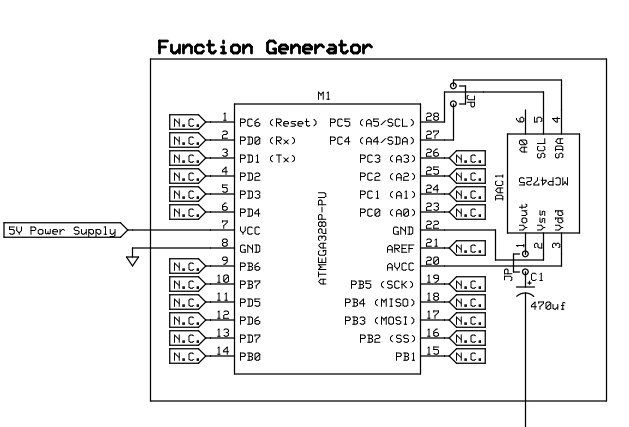
\includegraphics[width=3in]{./Function_generator.png}
	\caption{Function generator design with ATMEGA chip and MCP4725 DAC}
	\label{fig:function-generator}
\end{figure}

The DAC attenuates the $+5V \pm 10\%$ voltage supply from the Arduino UNO with $2^{12}$ individual output values. A peak-to-peak sawtooth voltage signal is the result, with a bit resolution of 1.2 mV/bit at a frequency of 2.5 Hz (see Figure~\ref{fig:five-volts-15-hz-wave}). However, due to the speed of the output of the DAC, 10 kHz, there is a substantial amount of noise which is filtered out in the next stage of the driver. The MCP4725 signal-generator acts as a near-perfect voltage source with a series impedance of $1\Omega$ when in normal operations. This will not affect input resistances for the analog design.  

\begin{figure}[h!]
  \centering
	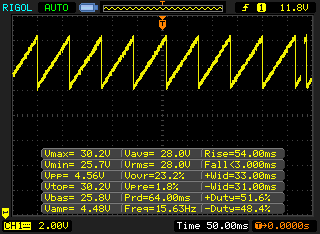
\includegraphics[width=3in]{./data/dac-output-waveform.png}
	\caption[Cavity Mounts]{The output of the MCP4725 DAC from the I2C communication with the Arduino which has 4096 individual steps from $0-5 \pm 10\% V$}
	\label{fig:five-volts-15-hz-wave}
\end{figure}

%---------------------------
% Analog-Amplifier Circuit
%---------------------------

\subsection{Analog-Amplifier Circuit}

The sawtooth waveform is sourced to a three-stage negative feedback amplifier, using LT1006 OpAmps, configuration (Figure~\ref{fig:amplifier-configuration}). The amplification ($A_v$) is adjustable from $0.1 V/V$ up to $9 V/V$. This is done through three stages: the dispersion stage and the two magnitude stages. The dispersion stage allows for small adjustments, 0.1x to 1x of the original signal based on $R_{in_{min}} = 10k\Omega$ and $R_{in_{max}} = 50k\Omega$. The magnitude stage allows for roughly 1x to 3x of the original signal based on  $R_{in_{min}} = 3.6k\Omega$ and $R_{in_{max}} = 10k\Omega$. Resistors R1, R2, and R3 are representation a resistor in series with a potentiometer. R1 is a $10k\Omega$ resistor in series with a $100k\Omega$ potentiometer. R2 and R3 are simply a $3.3k\Omega$ resistor in series with a $10k\Omega$ potentiometer. This was done for simplicity as the precision of the range was not a high priority. 

The overall gain ($A_v$) is adjustable because of these resistors and is governed by Eq.~\ref{eq:pot}.

\begin{equation}
A_v = (R_f)^3\Big(\frac{1}{R_1}\Big)\Big(\frac{1}{R_2}\Big)\Big(\frac{1}{R_3}\Big)
\label{eq:pot}
\end{equation}

A LTSpice Netlist program was developed (see code on page~\pageref{software:ltspice}). This provided the expected output of the signal given a specified input signal. This input signal is generated by a python-shell script which generates a PWL file for LTSpice.

This is sourced to a buffer which uses a single LT1006 (see Datasheet on page~\pageref{datasheet:lt1006}) operation amplifier. This gives the AC signal an infinite output impedance, preventing impedance mismatching. Figure~\ref{fig:buffer} denotes the circuit construction.

\begin{figure}[h!]
  \centering
	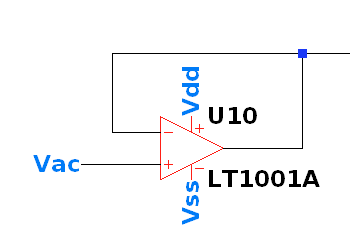
\includegraphics[width=3in]{./ltspice/unity-buffer-ltspice.png}
	\caption{The voltage follower (unity buffer amplifier) configuration for an OpAmp for circuit isolation and prevention of impedance mismatching.}
	\label{fig:buffer}
\end{figure}  

To change the offset biasing of the sawtooth voltage signal a LT3080 (see Datasheet on page~\pageref{datasheet:lt3080}) adjustable DC voltage regulator is added using a summation circuit to the AC signal with the following configuration (Figure~\ref{fig:dc-adj-voltage}).

\begin{figure}[h!]
  \centering
	\includegraphics[width=3in]{./schematics/dc-adj-voltage.png}
	\caption{DC adjustable voltage regulator for adjusting the DC offset of the signal}
	\label{fig:dc-adj-voltage}
\end{figure}  

%---------------------
% Power Distribution
%---------------------

\subsection{Power Distribution}

A VELLEMAN PSINO2512N 12-VOLT 25-WATT DC SWITCHING POWER SUPPLY (see Datasheet on page~\pageref{datasheet:psin02512n}) was complimented with a DROK Micro Electric DC/DC Boost Converter LM2577 Step-up Voltage Transformer (see Datasheet on page~\pageref{datasheet:lm2577}) to provide the power to the system. A LT1129 5 VDC $\pm 1\%$ fixed voltage regulator (see Datasheet on page~\pageref{datasheet:lt1129}) and an MAX737 inverting buck-boost converter (see Datasheet on page~\pageref{datasheet:max635}). 

The 12VDC PSIN02512N voltage supply is sourced to LM2577, boosting the voltage to 17 VDC. The 17 VDC is sourced to the LT1129 5-VDC producing +5 volts suppling power to the boot-loaded Arduino and the MCP4725 DAC. 

Since the design calls for a signal with a max peak-to-peak voltage of approximately 34V, the rails must have a range +17 VDC to -17 VDC. Since the constraint that $V_s - V_out \leq 22 V_DC$ holds for the buck converter, if the 5VDC rail is used, $V_{out_{max}} = -17 V$~\cite{MAX635}. This is achieved by using values for $R_3 = 82\;k\Omega$ and $R_4 = 1.06\;M\Omega$ (Figure~\ref{fig:max635}). 

\begin{figure*}[tb]
  \centering
	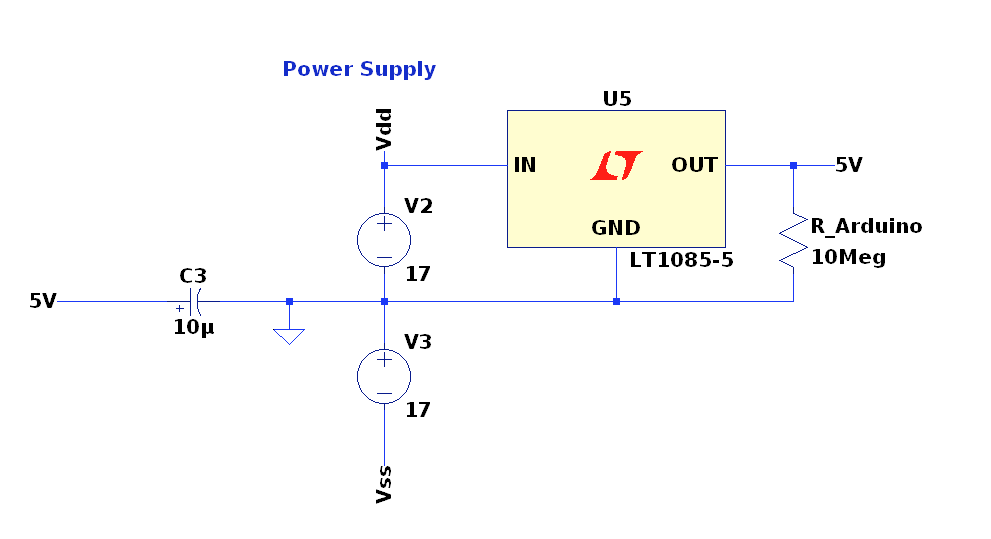
\includegraphics[width=6in]{/ltspice/power-supply-circuit-desgin-ltspice.png}
	\caption{This power supply setup allows for supplying the 17V rails necessary for the operational amplifiers as well as a 5V supply for the micro-controllers being used.}
	\label{fig:amplifier-configuration}
\end{figure*}

The current design of the board, which will be discussed later in this section, was simulated in LTspice for power consumption calculations. The total load of the system is simulated to be less than 30 mA. The current devices are rated well above this value, so loading issues should not be preset. The negative power supply was sinking 22.69 mA of current. In order to calculated the range of inductance and capacitance necessary for operations Eqs~\ref{eq:ipk} and~\ref{eq:l} were used. 

\begin{equation}
L_{min} = \frac{(1-D)^2 * R_{min}}{2*f}
\label{eq:ipk}
\end{equation}

\begin{equation}
C_{min} = \frac{D}{R_min*f*v_r}
\label{eq:l}
\end{equation}

Where $D = \frac{V_o}{V_o + V_s} = 0.77$ (duty cycle), $f = 50\text{kHz}$ (switching frequency), $R_{min} = 850\Omega$ (maximum load resistor), and $v_r = 0.01$ (ripple voltage). The minimum inductance was found to be $440\mu H$ and the minimum capacitance was found to be $1.82\mu F$. 

\begin{figure}
	\centering
	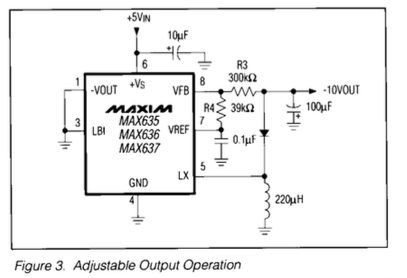
\includegraphics[width=3in]{./max635.png}
	\caption{Adjustable Output Operation~\cite{MAX635}}
	\label{fig:max635}
\end{figure}


% Analog Data Conversion Processor
%-----------------------------------------------------------------------------------------------------------------------------------

\section{Analog Data Conversion Processor}\label{processor}

The photodiode is mounted to an adjustable plate at the rear of the sFPI for calibration, for maximum transmission of the spectral content. The photodiodes resulting current is reverse biased by an Arduino UNO (\#2), which is supplying the 5V. Based on the IV curve of the photodiode, the voltage stays within the photo-conductive range while remaining far enough away from the breakdown voltage. 
\\\\
A recent Ph.D. thesis details the quantum efficiency of doped GaAs being between 30\% and 22\%~\cite{responsivity}. This means at 632.8 nm a good approximation for the responsivity is 154 mA/W. The incident power on the detector can be approximated based on the losses in the cavity. Section~\ref{ss:optical_design} explained that the reflectivity of the mirrors was between $99.4\% - 99.8\%$. From this the transmitted power of the beam can be calculated for one pass through the cavity:

\begin{equation}
P_{out} = T_1T_2*P_{in}
\end{equation}

Given the ranges for reflectivity given above, that $T = 1-R$, and $P_{in} = 3 mW$, the output power of the cavity was found to be $P_{max} = 0.108 \mu W$ and $P_{min} = 120 nW$. With an optical output of approximately $1\;\mu W$ results in a current of roughly $0.154\;\mu A$. However, it is wrong! This could be due to the photodiode not being consistent with the model or that my measurement of the optical power was incorrect. Whatever the case may be the diode current was experimentally determined to be roughly 1nA. 

\begin{figure*}
	\centering
	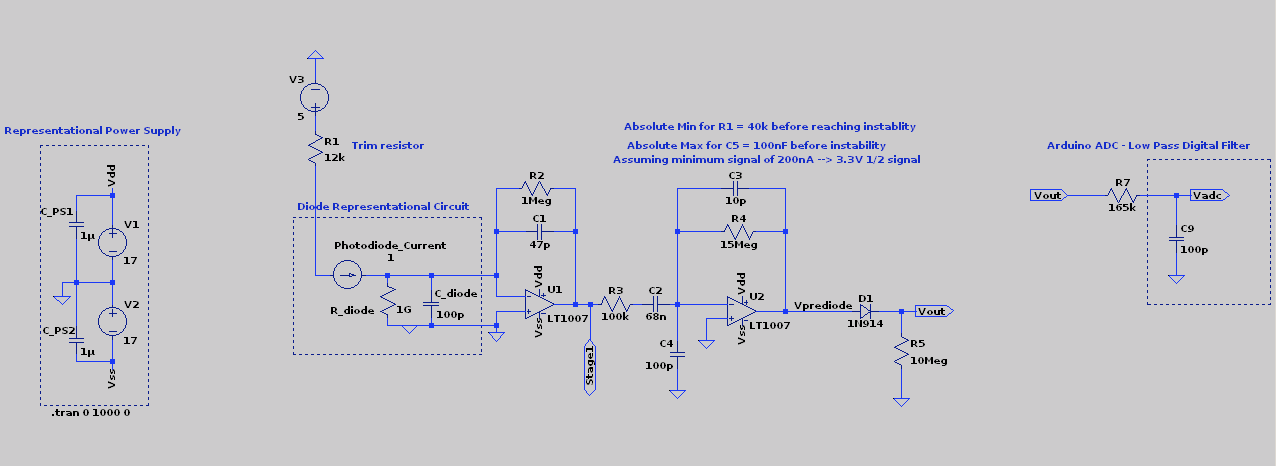
\includegraphics[width=\textwidth]{./transimpedance_amp_design.png}
	\caption{Trans-impedance amplifier design}
	\label{fig{transimpedance-amp}}
\end{figure*}

A trans-impedance negative-feedback amplifier with a voltage booster (TAV) converts the AC-current signal to a AC-voltage signal, which uses a AD8672 (see Datasheet on page~\ref{datasheet:ad8672}), The voltage gain of this amplifier setup is adjustable for tuning the sFPI, when the signal-to-noise ratio is small, to increase the intensity of the output of the cavity. This corresponding output is sampled by an analog-to-digital converter (ADC). Since the Arduino, the micro-controller used for storing the data, uses a prescaler of 128, the ADC clock speed is set at 125 kHz. Given that it takes 13 ADC clocks for a conversion the ADC can sample data at a rate of 9615 Hz. Since our we have 4096 individual steps, to match the rate of the ADC a frequency of 2.35 Hz in used for the driver.    

%---------------------------
% Digitally Analyzed Output
%---------------------------

\section{Digitally Analyzed Output}\label{digital-output}

The content captured by the ADC is transmitted to a computer to process, display (by a graphical representation), and stores the data by user command.  

%---------------------------
% ADC-Computer Interface
%---------------------------

\subsection{ADC-Computer Interface}

The voltage signal from the TAV is sampled by the Arduino UNO, as discussed in Section~\ref{processor}. This is converted to a 512 byte array. The array is then encoded to send to the computer upon request (see code in Section~\ref{serial-data}).

%---------------------------
% Data Analysis
%---------------------------

\subsection{Data Analysis}

This data will be combined in conjunction with the 5V sawtooth signal to plot the photodiode signal as a function of the geometrical change of the resonant cavity, which is proportional to the wavelength of the light. This will be done via a GUI model with a language that possesses the capability for universal interfacing. The current construct model is in Python and adequately provides a way to sample, view and store the data.

% Discussion and Conclusion
%-----------------------------------------------------------------------------------------------------------------------------------

\section{Discussion and Conclusion}

While the project in whole was not finished, the crucial parts of the design were completed as well as the optical and mechanical construction of the cavity and the sFPI driver. The resonant cavity was successfully integrated with mechanical design using adjustable mounting brackets and CNCed aluminum based and 3D printed parts. This allowed the user to align or misalign the cavity as desired. The mirror's separation can be modified to fit different parameter constraints. 

The construction of the sFPI driver was successful on the second iteration of the design. This iteration produced a sawtooth waveform output with amplitude ranging from 5V to 15V and a DC offset range of 0 to 28V (see Figures on page~\pageref{ss:output-signal-graphs}). While the first design did not meet the design parameters of the project, it created a stepping stone which further enhanced the finalized the design. The finalized design was simulated in LTSpice and produced the following output based on the best interpretation input of the DAC outputted. This re-design increases the amplitude range to 0.5V to 32V and the DC offset range from -17V to 17V (see Figures on page~\pageref{subss:final-design-output})\footnote{The reason that the DC offset changed from a low of 0 to -17V was the way the previous iteration was put together and tested. The output was connected across the $V_{out}$ and the $V-$, which is the reason a range from 0 to 28V was seen.}. It eliminated noise issues by creating a bandpass filter of the system as can be seen in the output of the LTSpice simulation.  

The trans-impedance amplifier system was not successfully constructed; however, the design and simulation was completed. The first two designs had the wrong bandpass filtering system as well as an incorrect overall closed loop gain. This was due to inaccurate measurements of the photodiode current when light was incident upon it. The final design takes into account a range of photodiode currents from 0 to 4 nA as well as a filtering system which passes through frequencies in the range 6Hz to 400Hz. This eliminates the majority of unwanted noise in the system. The design was also based around the Arduino UNO's digital filtering because of the slow sampling rate of the ADC (see Figures on page~\pageref{subss:trans-amp-output}).

The GUI application was designed; however, the algorithm for auto calibration is still incomplete. The GUI allows the user to select which serial port to use (cross platform compatible), calibrate the current input, as well the ability to start and stop taking data (see Figures on page~\pageref{subss:GUI}).   

% Discussion and Conclusion
%-----------------------------------------------------------------------------------------------------------------------------------

\section{Moving Forward}

In order to improve on the design, the sFPI driver could be tuned better in the frequency spectrum to produce a more polished signal. The trans-impedance amplifier and Arduino UNO sampling device need more work with syncing with the function generator as well as also producing a more polished signal. The GUI could be developed in a better platform (i.e. C++) and modeled to fit a Windows environment instead of a Apple. The mechanical design could be improved by having a micrometer base for precise knowledge of the distance between the two mirrors. Also by adding in a lens holder which is aligned with the first mirror would make aligning the cavity easier and quicker. The schematics still need to be finished in their design and creation. I used Eagle to create what is currently on the git repository; however, more accurate design for PCB development is needed. 

% Acknowledgments
%-----------------------------------------------------------------------------------------------------------------------------------

\section{Acknowledgments}

I could not have had the success I did without the help of my professors and academic colleges. Thanks go out to Dr. Scott Prahl for mentoring me on this project as well as suggesting the idea to me. I would like to thank the Optoelectronics program at OIT for making this project possible by providing all of the necessary parts that I needed for prototyping and construction. Thanks to Brandon Clarno for providing me with precision milling of the designs I provided him. He was instrumental in bringing the aluminum base to life as well as the first iteration of the piezo-mirror holder milled out of PVC plastic. Thanks go out to Caleb Schlamp for moral support and advisement of the electrical design. Thanks to Frank Rytkonen and Neils Williams for helping me construct a theoretically feasible power supply to power my design. 

% References
%-----------------------------------------------------------------------------------------------------------------------------------
\bibliography{OIT_Thesis}
%-----------------------------------------------------------------------------------------------------------------------------------

% Appendix
%-----------------------------------------------------------------------------------------------------------------------------------
\begin{appendices}
\onecolumn


% Output Signal Graphs
%-----------------------------------------------------------------------------------------------------------------------------------

\section{Data and Results} 

%---------------------------
% sFPI Driver - 2nd Design Iteration Output
%---------------------------
\subsection{sFPI Driver - 2nd Design Iteration Output} \label{ss:output-signal-graphs}

\begin{figure}[h!]
	\centering
	\includegraphics[width=\textwidth]{./data/max_amp_due_to_rails.png}
	\caption{With amplification at a maximum, the amplitude of the waveform was only able to reach 15Vpp. While is will work, it was only half of the desired range. The redesign, which still needs to be tested will produce a waveform with a range of 32V instead of 15V.}
	\label{fig:max-amp-2nd-iteration}
\end{figure}
\newpage

\begin{figure}[h!]
	\centering
	\includegraphics[width=\textwidth]{./data/dc_max_ramp.png}
	\caption{With the voltage regulator adding the maximum amount of DC voltage to the signal, the DC offset of the signal is 28V.}
	\label{fig:max-dc-offset}
\end{figure}
\newpage

%------------------------------------------------------
% sFPI Driver - Final Design Iteration LTSpice Output
%------------------------------------------------------
\subsection{sFPI Driver - Final Design Iteration LTSpice Output} \label{subss:final-design-output}

\begin{figure}[h!]
	\centering
	\includegraphics[width=\textwidth]{./ltspice/max-amplification.png}
	\caption{The final design allowed for an amplitude of the signal to reach 32Vpp.}
	\label{fig:max-amp-final-iteration}
\end{figure}
\newpage

\begin{figure}[h!]
	\centering
	\includegraphics[width=\textwidth]{./ltspice/min-amplification.png}
	\caption{The final design allowed for an amplitude of the signal to go as low as 500mVpp}
	\label{fig:min-amp-final-iteration}
\end{figure}
\newpage

\begin{figure}[h!]
	\centering
	\includegraphics[width=\textwidth]{./ltspice/fft-amplification.png}
	\caption{This eliminated most unnecessary noise in the system}
	\label{fig:fft-final-iteration}
\end{figure}
\newpage

%---------------------------------------------------------------------------
% sFPI Transimpedance Amplifier - Final Design Iteration LTSpice Output
%---------------------------------------------------------------------------
\subsection{sFPI Trans impedance Amplifier - Final Design Iteration LTSpice Output} \label{subss:trans-amp-output}

\begin{figure}[h!]
	\centering
	\includegraphics[width=\textwidth]{./ltspice/transimpedance-amp-output.png}
	\caption{The final design allows for the sampling of the spectral frequency content of the sFPI cavity.}
	\label{fig:trans-amp-output}
\end{figure}
\newpage

\begin{figure}[h!]
	\centering
	\includegraphics[width=\textwidth]{./ltspice/transimpedance-amp-bandpass.png}
	\caption{The final design allows for the sampling of the spectral frequency content of the sFPI cavity eliminating noise.}
	\label{fig:trans-amp-fft}
\end{figure}
\newpage

%---------------------------------------------------------------------------
% sFPI GUI - Final Design Iteration Application
%---------------------------------------------------------------------------
\subsection{sFPI GUI - Final Design Iteration Application} \label{subss:GUI}

\begin{figure}[h!]
	\centering
	\includegraphics[width=\textwidth]{./GUI/main-screen.png}
	\caption{The GUI design allows the user to view the data live on the screen as it is sampled from the Arduino UNO.}
	\label{fig:GUI-main-screen}
\end{figure}
\newpage

\begin{figure}[h!]
	\centering
	\includegraphics[width=\textwidth]{./GUI/serial-port.png}
	\caption{This allows the user to change the serial port they want to use to collect the data from.}
	\label{fig:GUI-serial-port}
\end{figure}
\newpage

\begin{figure}[h!]
	\centering
	\includegraphics[width=\textwidth]{./GUI/calibrate.png}
	\caption{This allows the user to calibrate the system based on the input from the Ardunio UNO.}
	\label{fig:GUI-calibrate}
\end{figure}
\newpage

\begin{figure}[h!]
	\centering
	\includegraphics[width=\textwidth]{./GUI/menu-bar.png}
	\caption{The menu bar allows the user to pick from a select list of functions and operations to utilize on the data.}
	\label{fig:GUI-menu-bar}
\end{figure}
\newpage

\begin{figure}[h!]
	\centering
	\includegraphics[width=\textwidth]{./GUI/tools.png}
	\caption{This is the only menu bar that has been developed for use.}
	\label{fig:GUI-tools}
\end{figure}

\newpage


% Software Programs
%-----------------------------------------------------------------------------------------------------------------------------------

%---------------------------
% Arduino Programs
%---------------------------
\section{Arduino Programs} \label{software:arduino}

\subsection{Writing to the MCP4725 12-bit DAC via I2C}

\arduinoexternal{../App/Arduino/sFPI-driver/sFPI-driver.ino}

\subsection{Program for capturing and sending serial data to the computer} \label{serial-data}

\arduinoexternal{../App/Arduino/Serial-data/Serial-data.ino}


%---------------------------
% Python Programs
%---------------------------
\section{Python GUI} \label{software:python}

\subsection{Main program}
\pythonexternal{../App/GUI.py}

\subsection{Application Class}
\pythonexternal{../App/Application.py}

\subsection{USB Interface Class}
\pythonexternal{../App/USBInterface.py}

\subsection{GUI Errors Class}
\pythonexternal{../App/GUIErrors.py}

\subsection{Setup Function}
\pythonexternal{../App/setup.py}

\newpage


%---------------------------
% LTSpice Programs
%---------------------------
\section{LTSpice Netlists}\label{software:ltspice}

\subsection{Interferometer Driver LTSpice Netlist for Simulation}
\ltspiceexternal{../Electrical_Design/Amplifier_Design/Rev_2.0/amplifier_setup_rev2.txt}
\newpage

\subsection{Interferometer Trans-impedance Amplifier LTSpice Netlist for Simulation}
\ltspiceexternal{../Electrical_Design/Photodiode_Amplifier/transimpedance_amplifier.txt}

\newpage


% Mechanical Assembly Drawings
%-----------------------------------------------------------------------------------------------------------------------------------

\section{Mechanical Assembly Drawings}

%---------------------------
% PZT-Mirror Holder
%---------------------------
\subsection{PZT-Mirror Holder}

\begin{figure}[h!]
  \centering
	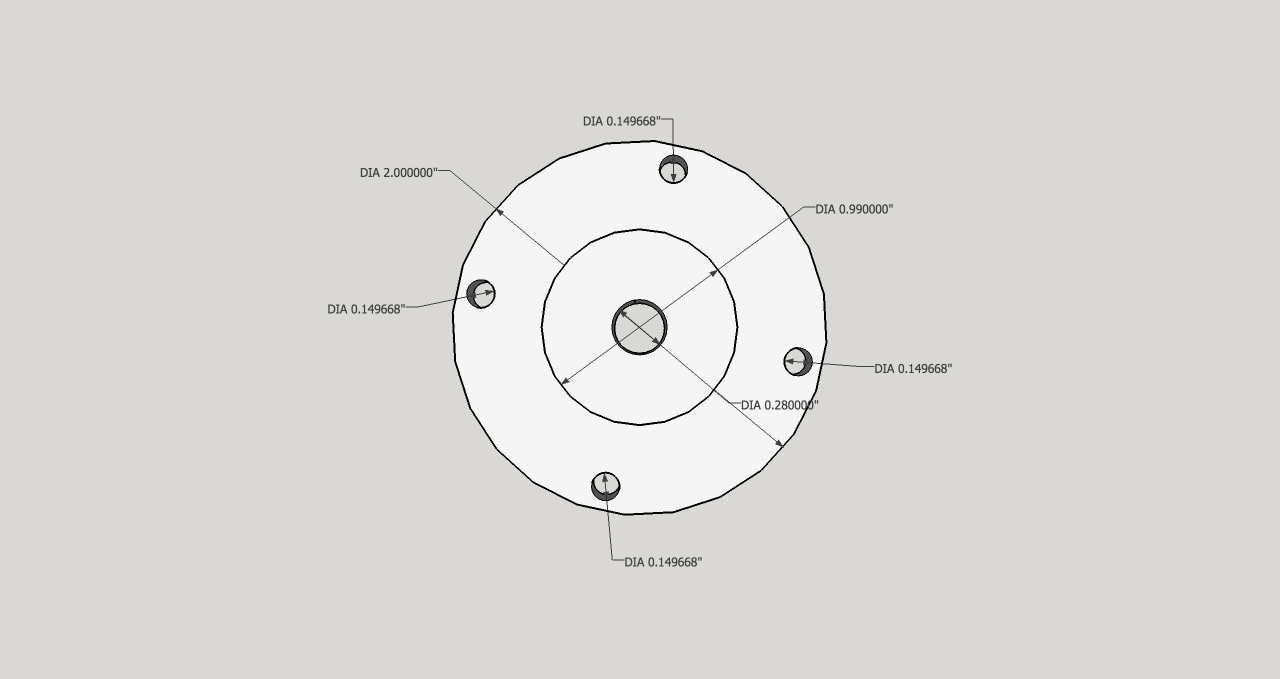
\includegraphics[width=\textwidth]{./mechanical/PZT_holder_top.png}
	\caption[Cavity Mounts]{The top down view and measurements of the PZT-Mirror holder}
	\label{fig:PZT-holder-top}
\end{figure}  
\newpage

\begin{figure}[h!]
  \centering
	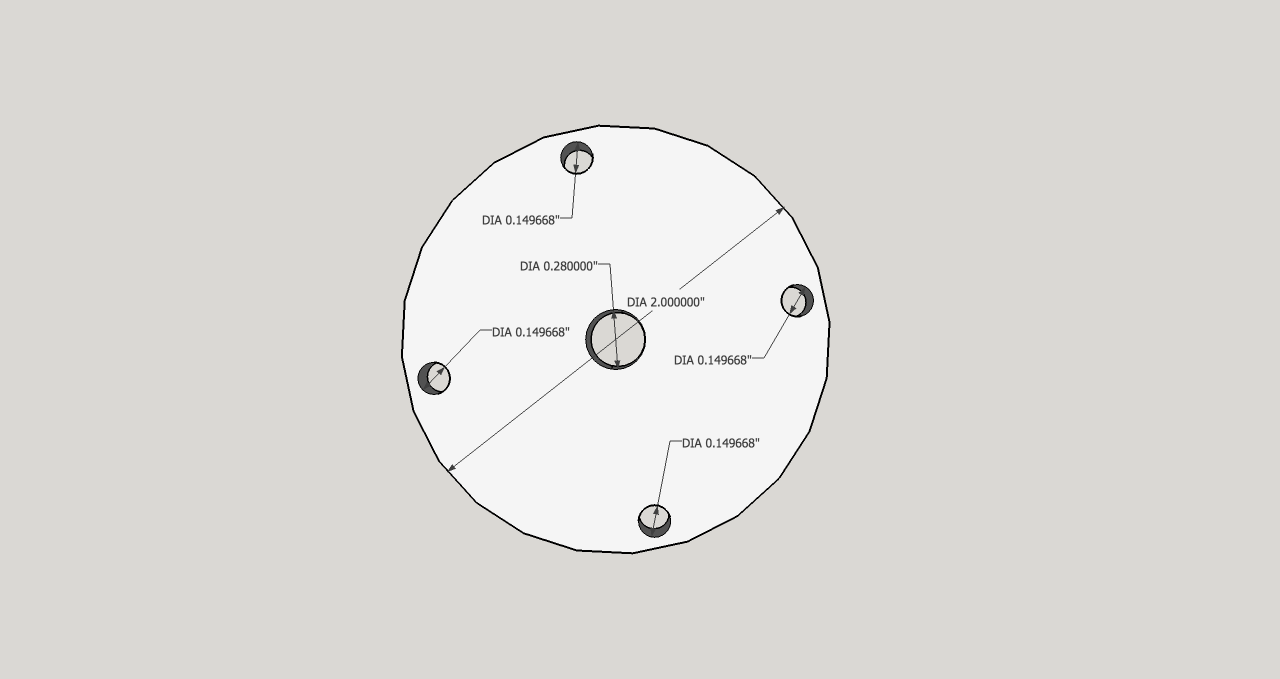
\includegraphics[width=\textwidth]{./mechanical/PZT_holder_bottom.png}
	\caption[Cavity Mounts]{The bottom up view and measurements of the PZT-Mirror holder}
	\label{fig:PZT-holder-bottom}
\end{figure}  
\newpage

\begin{figure}[h!]
  \centering
	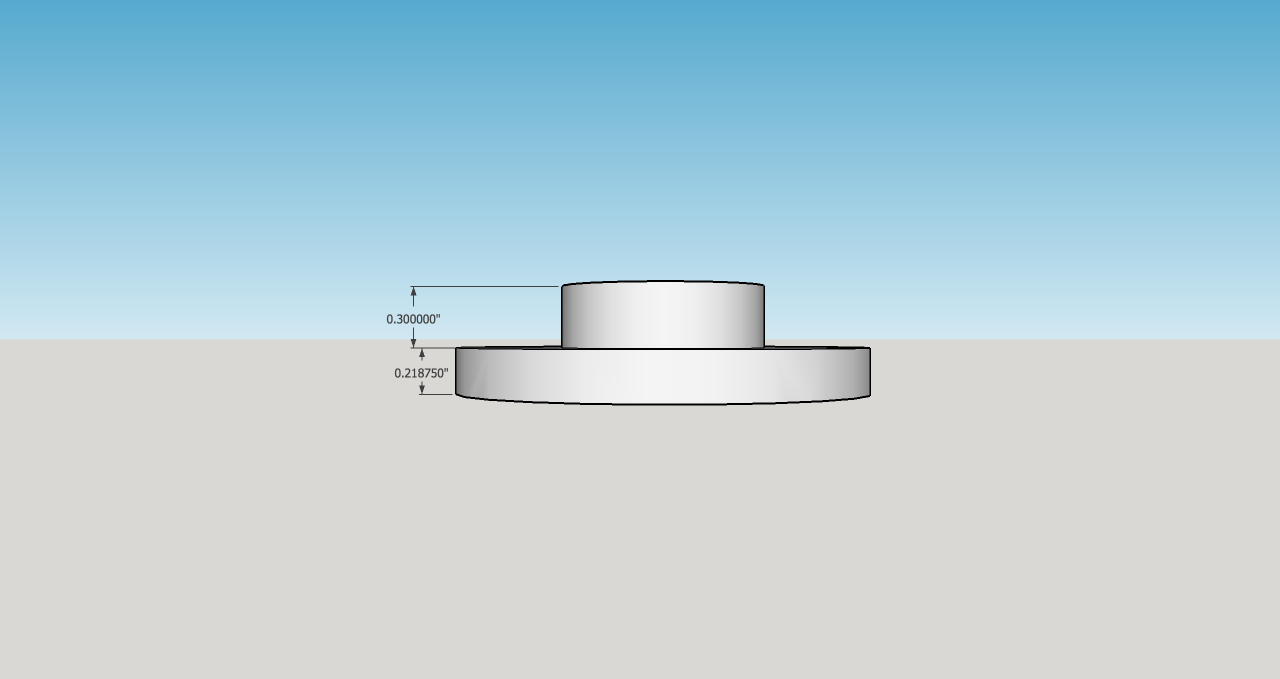
\includegraphics[width=\textwidth]{./mechanical/PZT_holder_side.png}
	\caption[Cavity Mounts]{The side view and measurements of the PZT-Mirror holder}
	\label{fig:PZT-holder-side}
\end{figure}  

\newpage

%---------------------------
% Aluminum Base
%---------------------------
\subsection{sFPI Aluminum Base} \label{ss:sfpilensholder}

\begin{figure}[h!]
  \centering
	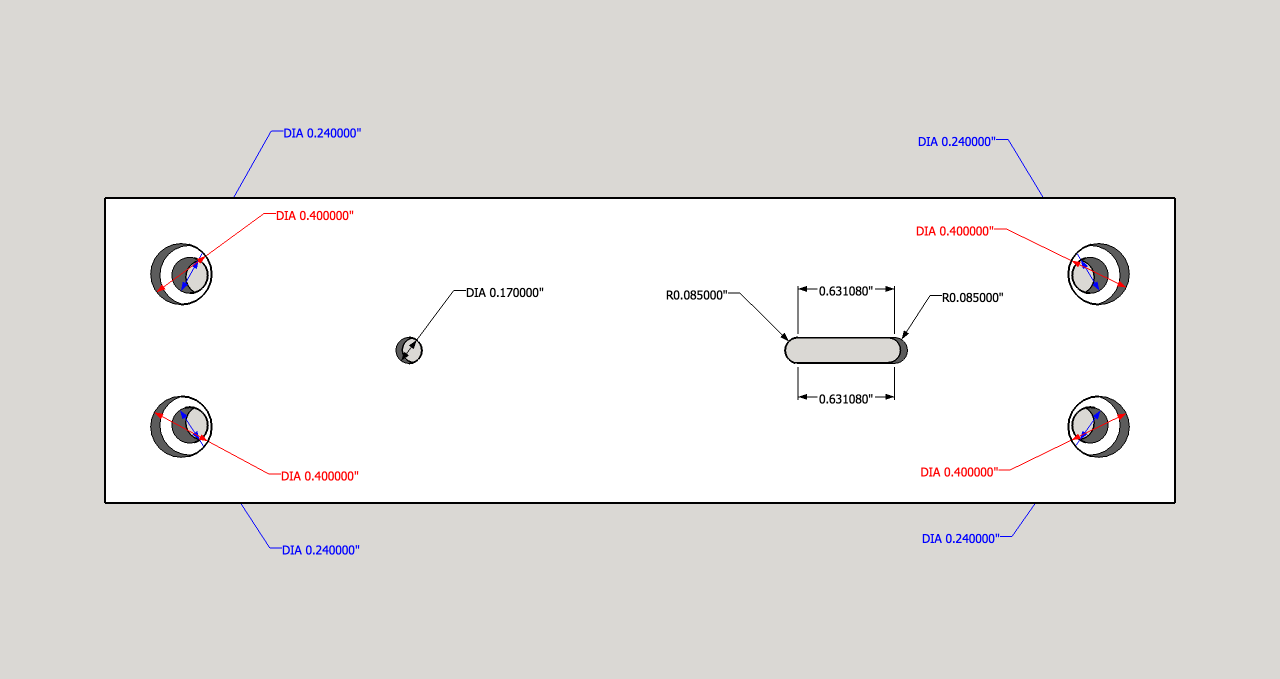
\includegraphics[width=\textwidth]{./mechanical/sfpilensholder_top.png}
	\caption[Cavity Mounts]{The top down view and measurements of the sFPI aluminum base}
	\label{fig:sfpilensholder-top}
\end{figure}  
\newpage

\begin{figure}[h!]
  \centering
	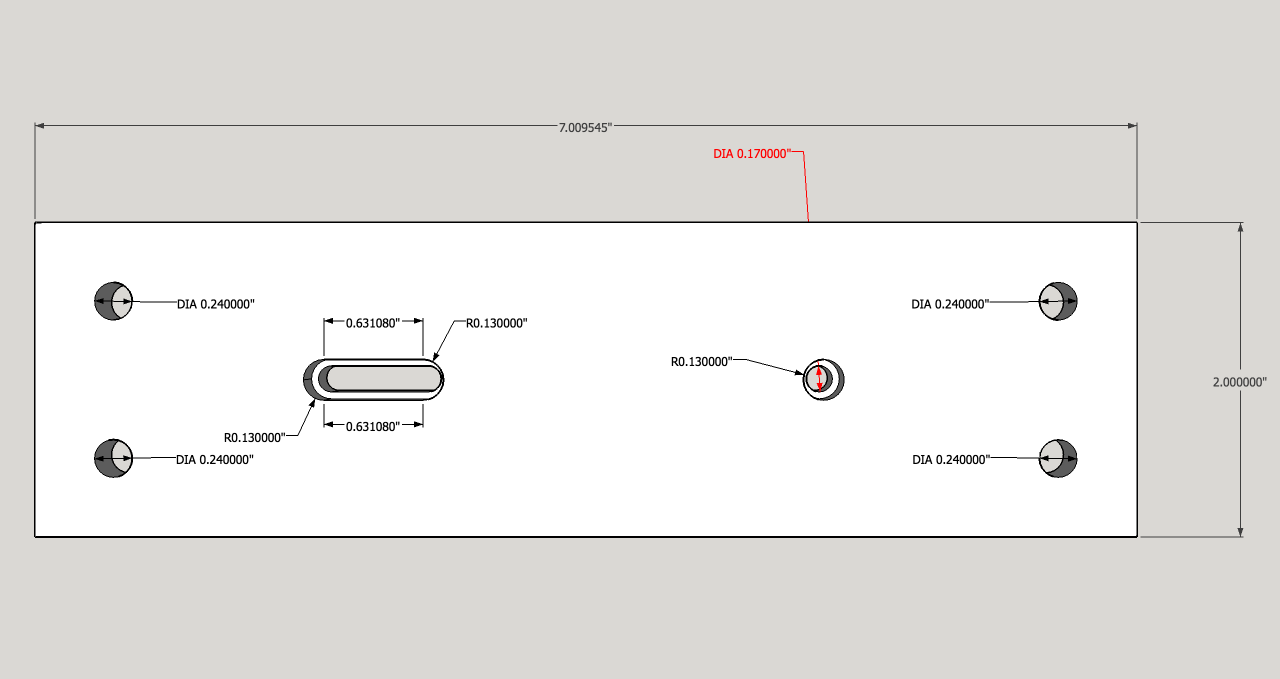
\includegraphics[width=\textwidth]{./mechanical/sfpilensholder_bottom.png}
	\caption[Cavity Mounts]{The bottom up view and measurements of the sFPI aluminum base}
	\label{fig:sfpilensholder-bottom}
\end{figure}  
\newpage

\begin{figure}[h!]
  \centering
	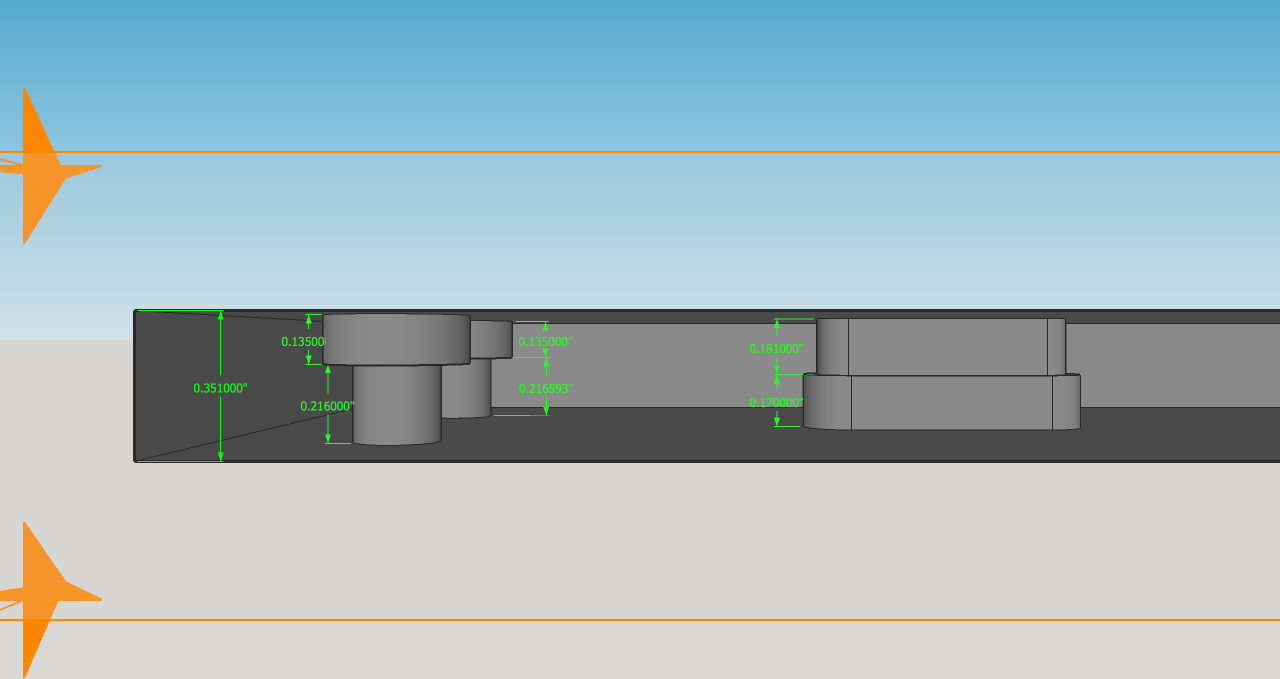
\includegraphics[width=\textwidth]{./mechanical/sfpilensholder_cross_section_1.png}
	\caption[Cavity Mounts]{The front cross section view and measurements of the sFPI aluminum base}
	\label{fig:sfpilensholder-side}
\end{figure} 
\newpage

\begin{figure}[h!]
  \centering
	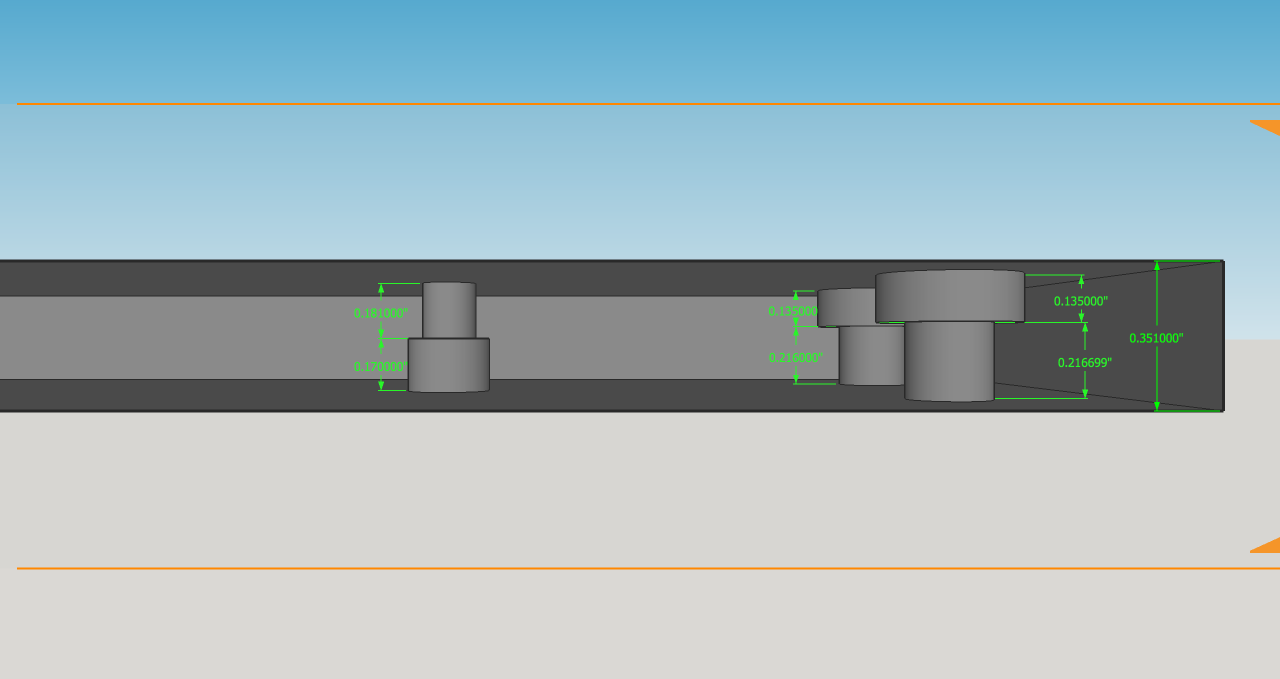
\includegraphics[width=\textwidth]{./mechanical/sfpilensholder_cross_section_2.png}
	\caption[Cavity Mounts]{The back cross section view and measurements of the sFPI aluminum base}
	\label{fig:sfpilensholder-side}
\end{figure}   

\newpage

%---------------------------
% Photodiode Holder
%---------------------------
\subsection{Photodiode Holder} \label{ss:diode_holder}

\begin{figure}[h!]
  \centering
	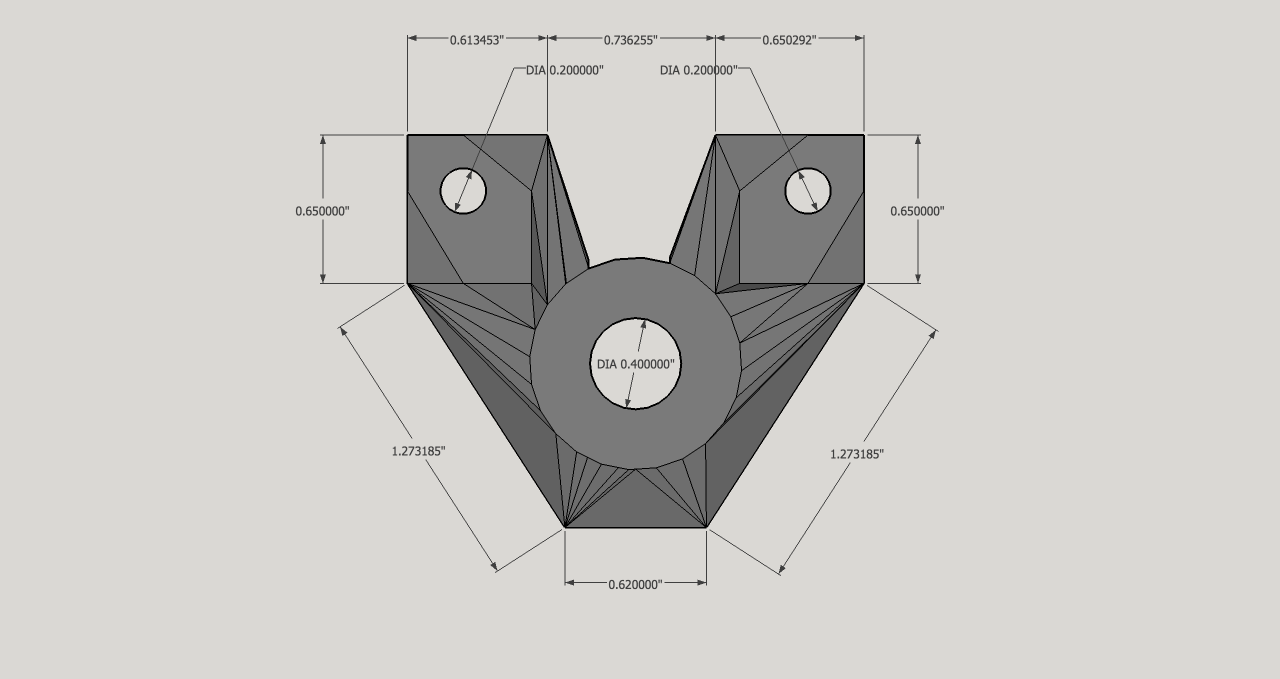
\includegraphics[width=\textwidth]{./mechanical/diode_holder_top.png}
	\caption[Cavity Mounts]{The top down view and measurements of the sFPI aluminum base}
	\label{fig:diode_holder-top}
\end{figure}  
\newpage

\begin{figure}[h!]
  \centering
	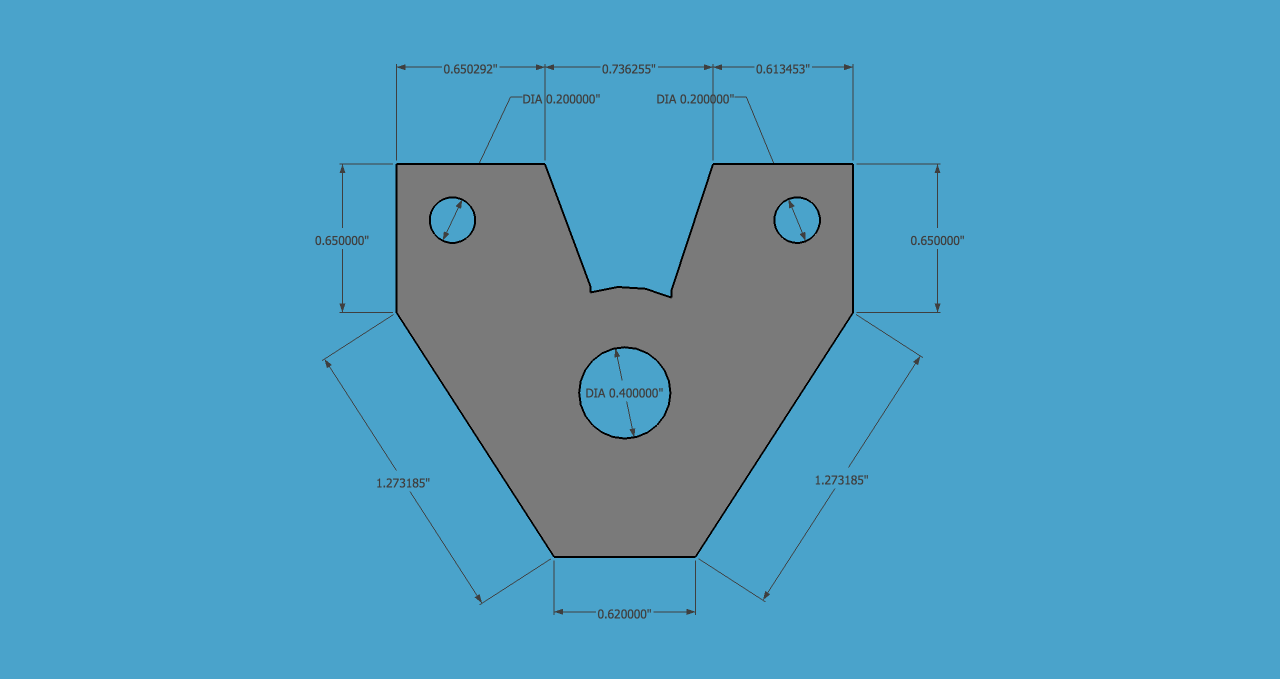
\includegraphics[width=\textwidth]{./mechanical/diode_holder_bottom.png}
	\caption[Cavity Mounts]{The bottom up view and measurements of the sFPI aluminum base}
	\label{fig:diode_holder-bottom}
\end{figure} 
\newpage 

\begin{figure}[h!]
  \centering
	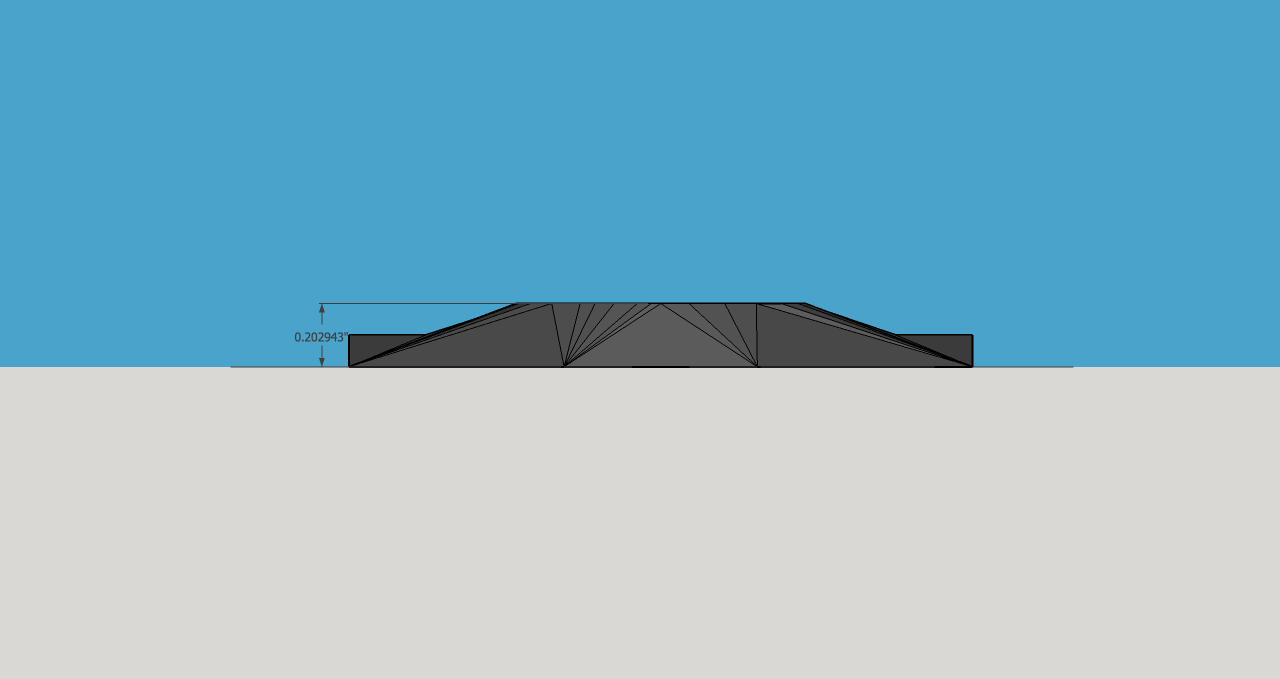
\includegraphics[width=\textwidth]{./mechanical/diode_holder_front.png}
	\caption[Cavity Mounts]{The front cross section view and measurements of the sFPI aluminum base}
	\label{fig:diode_holder-front}
\end{figure} 
\newpage

\begin{figure}[h!]
  \centering
	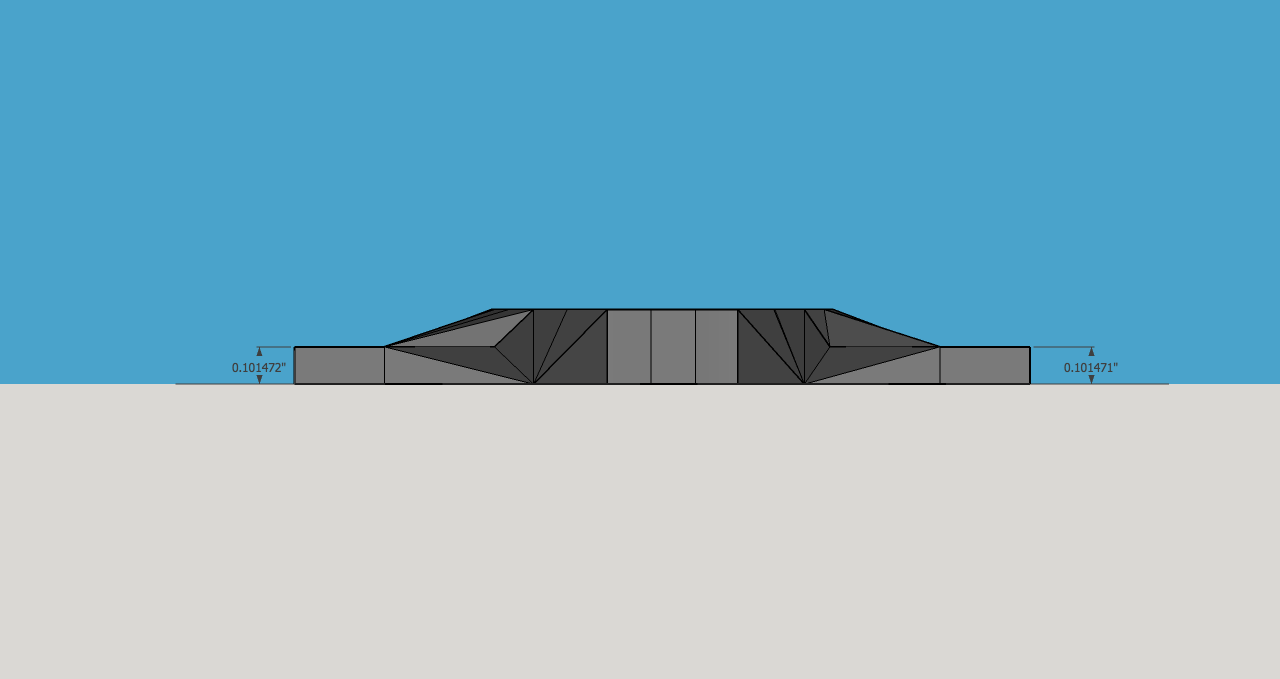
\includegraphics[width=\textwidth]{./mechanical/diode_holder_back.png}
	\caption[Cavity Mounts]{The back cross section view and measurements of the sFPI aluminum base}
	\label{fig:diode_holder-back}
\end{figure}  
\newpage

\begin{figure}[h!]
  \centering
	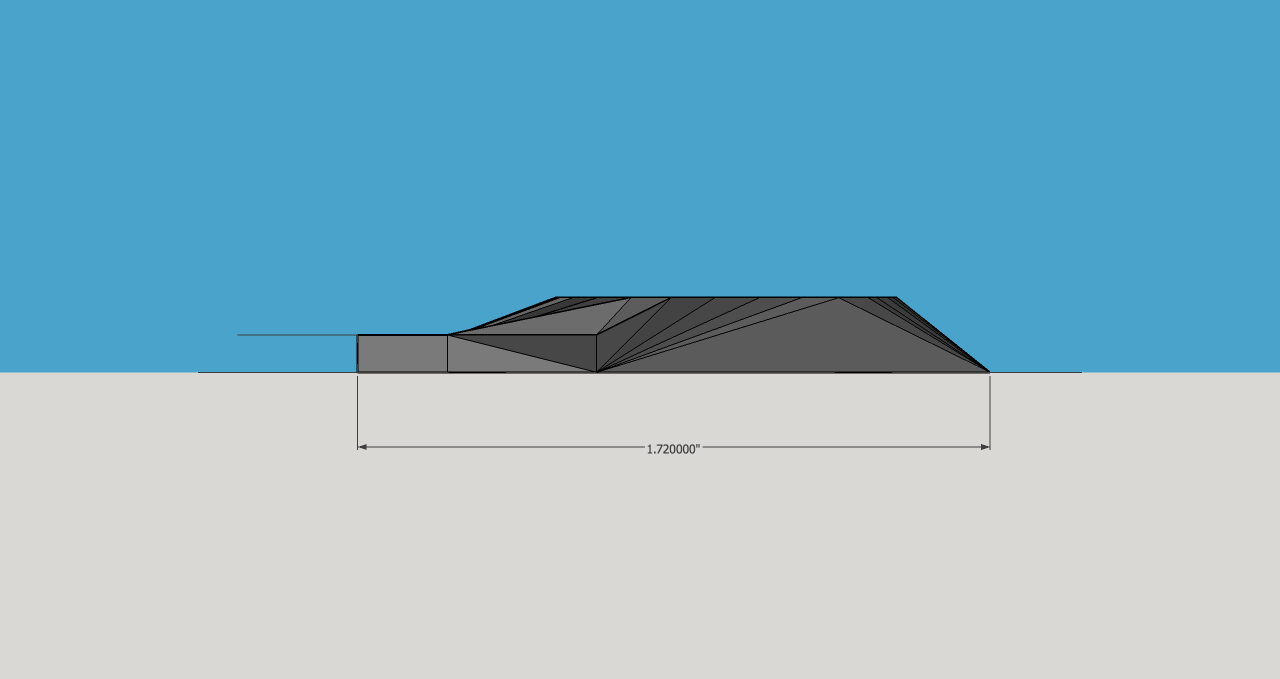
\includegraphics[width=\textwidth]{./mechanical/diode_holder_side.png}
	\caption[Cavity Mounts]{The back cross section view and measurements of the sFPI aluminum base}
	\label{fig:diode_holder-side}
\end{figure}   

\newpage

% Datasheets
%-----------------------------------------------------------------------------------------------------------------------------------

\section{Datasheets}

% ATMega 328P
\includepdf[pages=1-15]{../Datasheets/ATmega328.pdf} \label{datasheet:atmega328p}

% LT3080
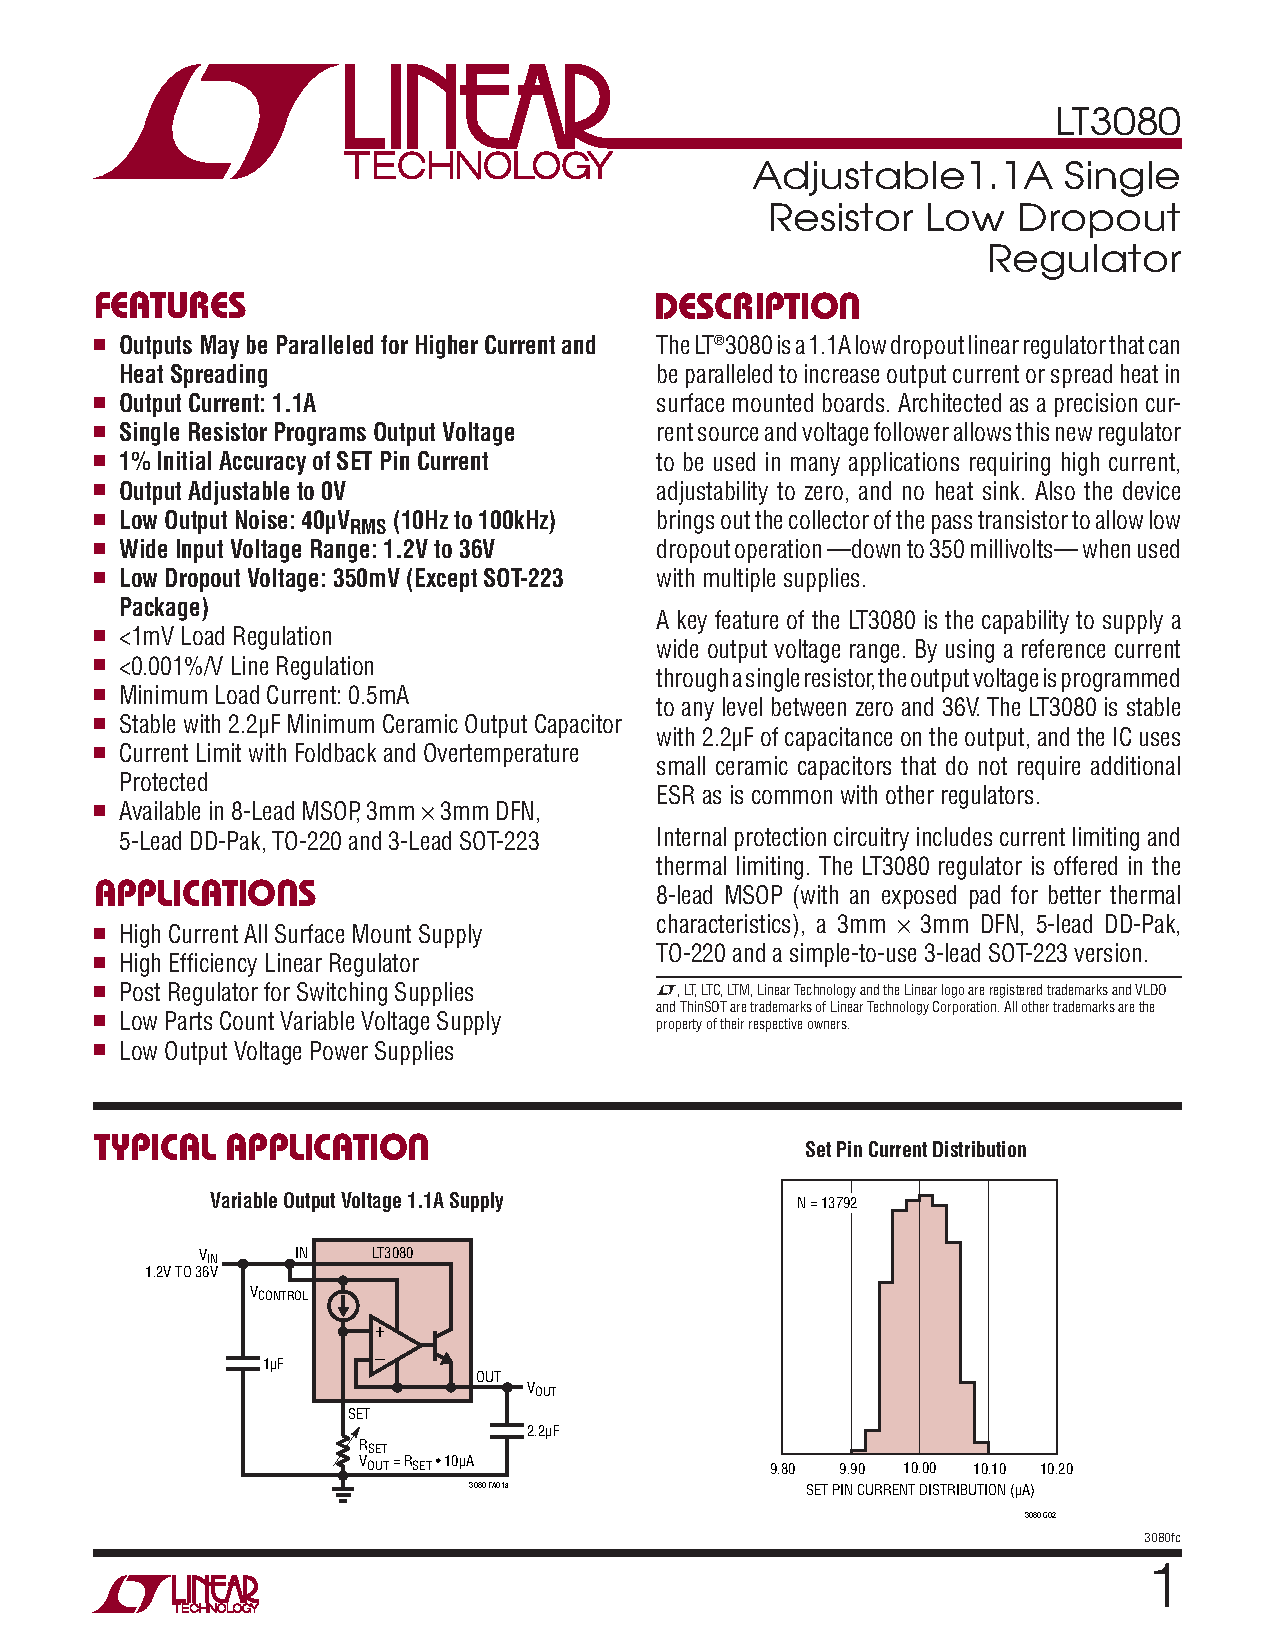
\includepdf[pages=1-15]{../Datasheets/LT3080.pdf} \label{datasheet:lt3080}

% LT1129-5
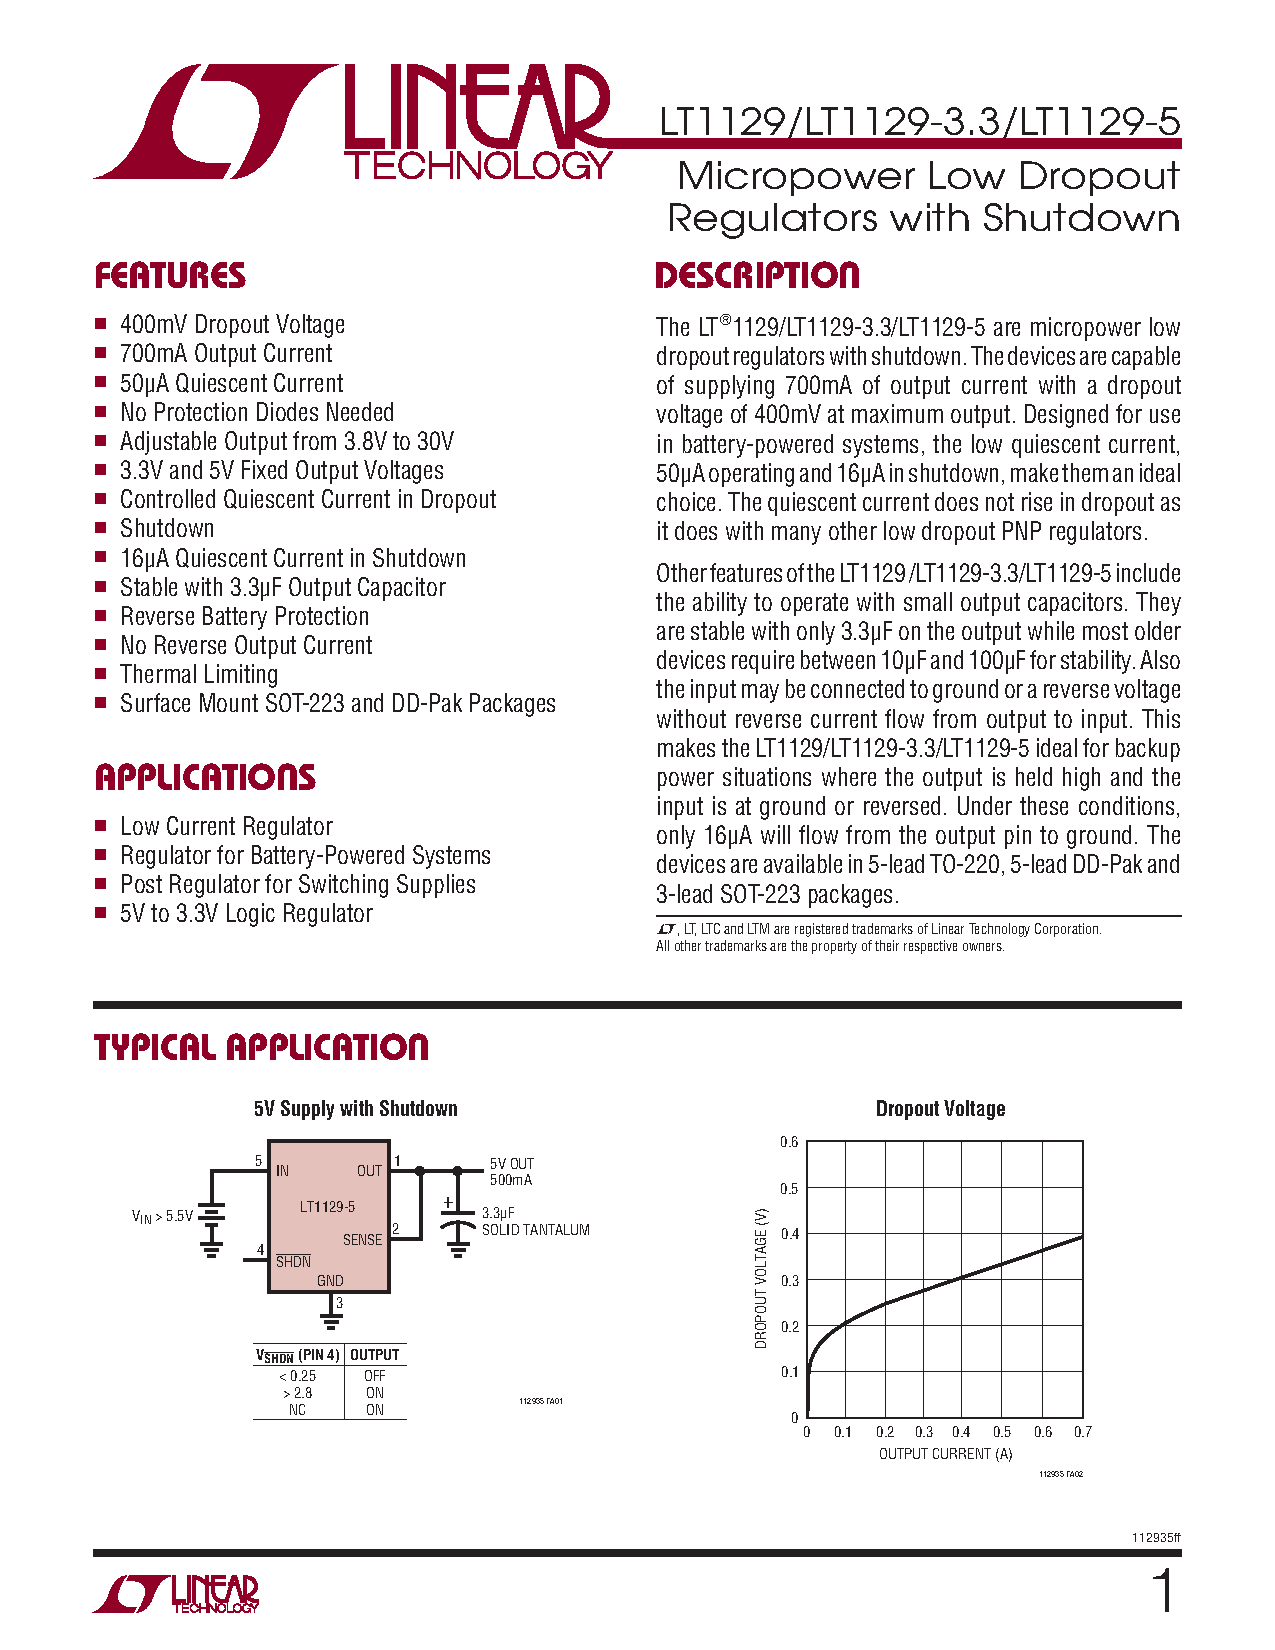
\includepdf[pages=1-15]{../Datasheets/LT1129-5.pdf} \label{datasheet:lt1129}

% MAX635
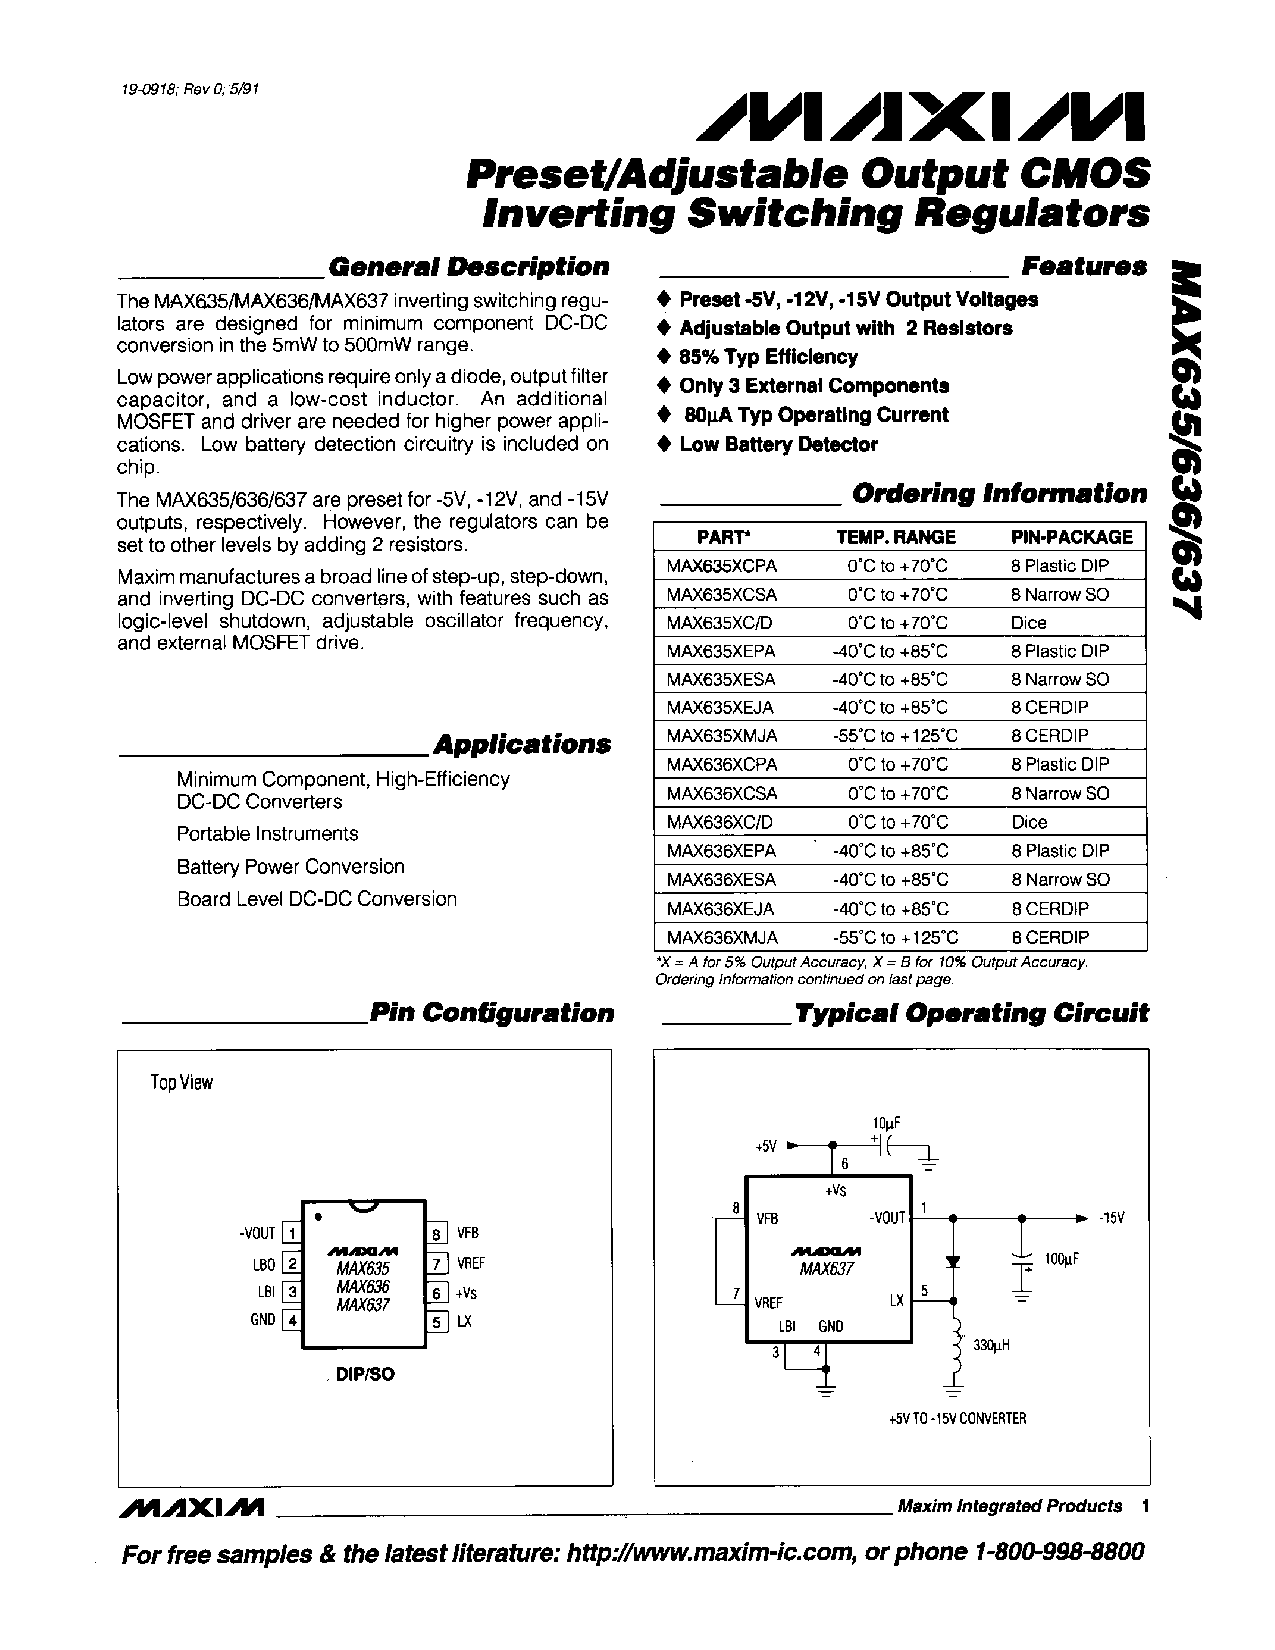
\includepdf[pages=-]{../Datasheets/MAX635.pdf} \label{datasheet:max635}

% LT1006
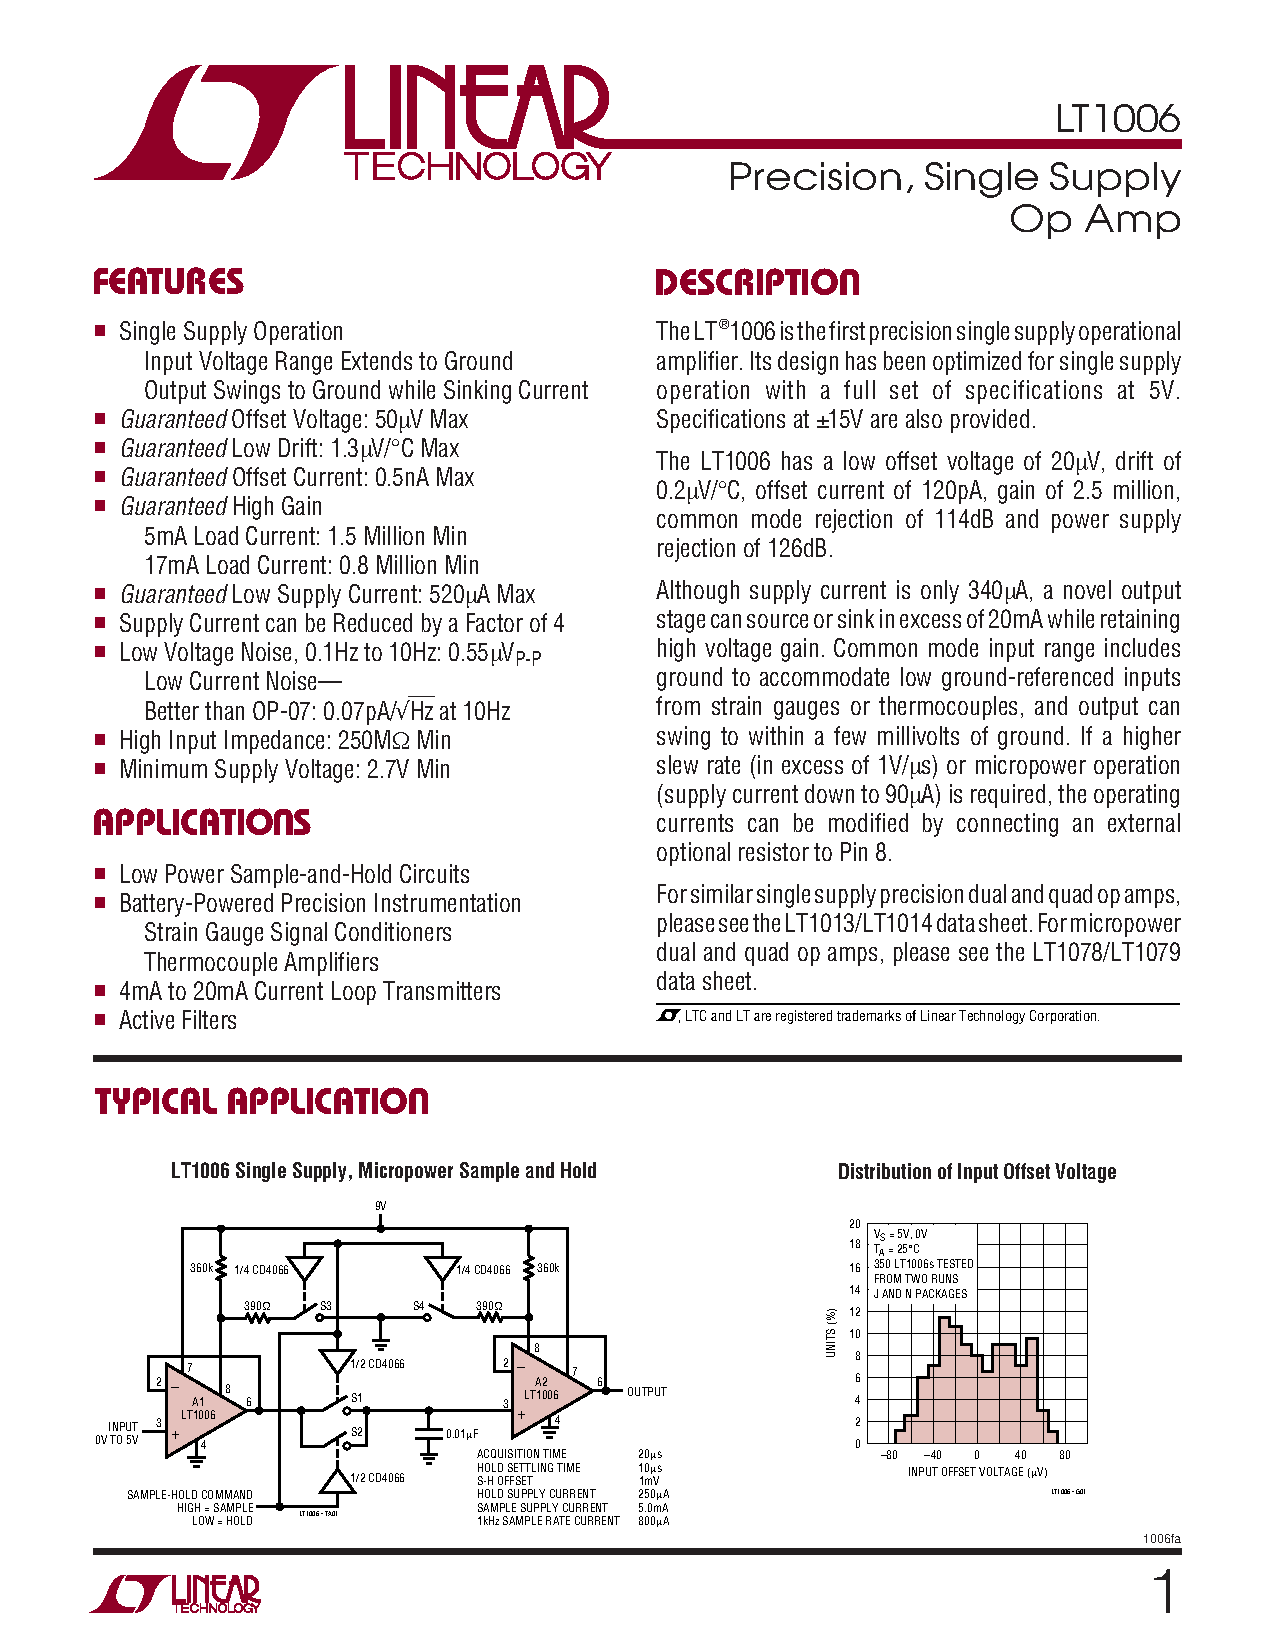
\includepdf[pages=-]{../Datasheets/LT1006.pdf} \label{datasheet:lt1006}

% MCP4725
\includepdf[pages={1,3-5,13,15-17}]{../Datasheets/mcp4725.pdf} \label{datasheet:mcp4725}

% Arduino UNO
\includepdf[pages=-]{../Datasheets/arduino_uno.pdf} \label{datasheet:arduino_uno}

% LM2577
\includepdf[pages=-]{../Datasheets/LM2577.pdf} \label{datasheet:lm2577}

% PSIN02512N
\includepdf[pages=-]{../Datasheets/PSIN02512N.pdf} \label{datasheet:psin02512n}

% AD8627
\includepdf[pages=-]{../Datasheets/AD8672.pdf} \label{datasheet:ad8627}

\end{appendices}

\end{document}
